% =====================================================================
% skarm — journal-quality paper (two-column, 10pt; results for all
% 25 datasets from the completed PC campaign, 2026-10-30)
% ---------------------------------------------------------------------
% STATUS: Final results version. Every measured number is filled by
% build_paper.py from benchmarks/cells/*.json plus the merged
% campaign_results.json — nothing hand-typed, nothing invented, no VM
% trial records merged in (different machine, different ladder).
%
% PLACEHOLDERS (filled by build_paper.py, in order):
%  P1  Abstract headline finding (one sentence, from the merged report)
%  P2  Section 6.2 condensed timing table (primary threshold only;
%      full cell table is Appendix B, P11)
%  P3  Section 6.2 result charts (runtime, memory, scatter, throughput,
%      itemsets, outcomes — all from the cell files)
%  P4  Section 6.2 correctness verdicts table (trial-0 agreement)
%  P5  Section 6.2 skips/timeouts table (with reasons, never hidden)
%  P6  Section 6.3 empirical trade-off discussion (from P2-P5)
%  P7  Section 8 headline conclusion sentence (from P2-P5)
%  P8  Appendix A: results commit SHA + machine spec (from JSON metadata)
%  P9  Confirm all 25 dataset files are present in repo data/
%  P10 Section 4 dataset-family pie (from Table 2's Type column)
%  P11 Appendix B: full per-cell timing table (all thresholds, engines)
% Author order per user 30 Oct 2026: Ramya, Anvitha, Abhishek Kumar,
% Giridhar, Rajeev (supervisor first; Abhishek third overall).
% TODO (before submission): re-check scikit-mine activity, mlxtend
%   version, and the two references marked [VERIFY] in the bibliography.
% =====================================================================
\documentclass[twocolumn,10pt]{article}
\usepackage[a4paper,margin=2.5cm]{geometry}
\usepackage{amsmath,amssymb}
\usepackage{booktabs}
\usepackage{longtable}
\usepackage{graphicx}
\usepackage{tikz}
\usetikzlibrary{arrows.meta,positioning,shapes.geometric}
\usepackage{xcolor}
\usepackage[hidelinks]{hyperref}
\setlength{\emergencystretch}{2em}

\newcommand{\placeholder}[1]{%
  \begin{center}
  \fbox{\parbox{0.9\textwidth}{\centering\textit{[PLACEHOLDER --- #1]}}}
  \end{center}}
\newcommand{\skarm}{\textsf{skarm}}

\title{\skarm: A scikit-learn-Compatible Estimator for Association-Rule
Mining with Auditable Pruning}
\author{
  Ms.~Dudigam Ramya\textsuperscript{1},
  Gontla Venkata Anvitha\textsuperscript{1},
  Abhishek Kumar\textsuperscript{1} \\
  Kamma Giridhar\textsuperscript{1},
  Paladagula Venkata Rajeev\textsuperscript{1} \\
  \small\textsuperscript{1}Department of Computer Science and Engineering,
  KL University, Vijayawada, India \\
  \small Capstone project KLCAP-2026-00340
}
\date{}

\begin{document}
\twocolumn[\maketitle

\begin{abstract}
Frequent-itemset mining and association-rule mining are standard tools
for market-basket analysis, recommendation, and categorical pattern
discovery, yet current scikit-learn offers no native estimator for them:
the feature request (issue \#32712) was closed as ``not planned'' on
scope grounds, with maintainers directing the work to a separate,
scikit-learn-compatible library. The closest existing library,
mlxtend, provides the mining functions but not an estimator API, and it
provides no Eclat. We present \skarm, a Python library that packages
three classic miners --- Apriori, FP-Growth, and Eclat --- behind a
single scikit-learn-style estimator with deterministic rule ordering,
explicit candidate-count telemetry, and a bounded-generation mode that
reports truncation instead of silently returning partial results. The
evaluation protocol compares all three engines plus an mlxtend baseline
at matched support thresholds on 25 datasets, with a 30-trial
statistical protocol on an 8-dataset subset and exact itemset-agreement
checks on every cell.
Across 25 datasets (1650 trial records on one Windows PC), all 157 compared engine pairs agree exactly on frequent itemsets; at each dataset's primary threshold, apriori fastest on none; fpgrowth fastest on 5 of 25; eclat fastest on 20 of 25, and mlxtend could not run 6 cells for stated reasons (3 dense-cap skips, 3 empty-input errors).
\end{abstract}
]

\section{Introduction}

\subsection{Problem}
Association-rule mining finds patterns of the form $X \Rightarrow Y$
over transactions, where $X$ and $Y$ are disjoint itemsets. The task is
unsupervised: unlike classification, there is no target variable, and
the output is a set of patterns whose size can explode combinatorially
as the support threshold falls. Any library that offers this task must
therefore answer three questions honestly: \emph{which} patterns were
found, \emph{whether} the output is complete, and \emph{what} it cost.
Most teaching implementations answer none of them.

\subsection{The scikit-learn scope story, stated honestly}
In November 2025 a community member asked scikit-learn for a native
Apriori estimator (issue \#32712 \cite{sklearn32712}), proposing a new
\texttt{sklearn.association} module with \texttt{fit()} for frequent
itemsets and rule generation with support, confidence, lift, and
leverage. The maintainers closed the request on 16 November 2025 as
``not planned'', ruling that pattern mining sits outside the scope of
machine learning as defined in scikit-learn, and suggested the work
belonged in scikit-mine or scikit-learn-contrib. An earlier discussion
(\#2662, 2013--2014 \cite{sklearn2662}) had reached the same conclusion. \skarm therefore
does not claim to implement a requested scikit-learn feature, and it
does not claim sklearn endorsement. It follows the maintainers' advice:
a separate library that is \emph{compatible} with scikit-learn's API
conventions (estimator with \texttt{fit}, fitted attributes with a
trailing underscore, parameter inspection), so it can sit beside
scikit-learn pipelines rather than inside them.

\subsection{Capstone objectives}
This work is the KL University capstone project KLCAP-2026-00340. Its
objectives, as registered in the portal specification, are: (O1) build
an Apriori baseline; (O2) add FP-Growth and Eclat behind one estimator;
(O3) make pruning auditable through candidate counts and a bounded
mode; (O4) verify correctness against independent implementations; and
(O5) evaluate on a broad, documented dataset collection. The portal
contract additionally requires a held-out partition reserved before
tuning (acceptance criterion AC-3), negative tests NT-1 to NT-6, and
KPI evidence including a 30-trial statistical protocol (KPI-4) and a
frozen two-rater rubric (KPI-2); Section~\ref{sec:setup} maps each
requirement to its evidence.

\subsection{Contributions}
\begin{itemize}
  \item One estimator, three engines: Apriori, FP-Growth, and Eclat
  with identical inputs, outputs, and rule metrics, so comparisons are
  between algorithms, not between APIs.
  \item Auditability by default: deterministic rule ordering, peak
  candidate counts, a degraded-mode flag with truncation counts, and
  recall against the exact result whenever bounded mode is used.
  Bounded output is never presented as exact.
  \item A documented 25-dataset evaluation collection with measured
  statistics and provenance for every file (Section~\ref{sec:data}),
  and a benchmark protocol (Section~\ref{sec:setup}) whose thresholds,
  trial counts, timeout rule, and correctness gate are fixed before the
  results are read.
\end{itemize}

\section{Related work}

\subsection{Classic algorithms}
Apriori \cite{agrawal1994} mines level by level, generating candidates
from the frequent itemsets of the previous level and pruning with the
anti-monotone property: every subset of a frequent itemset is frequent,
so any superset of an infrequent itemset can be discarded without
counting. FP-Growth \cite{han2000,han2004} compresses the database into
an FP-tree in two scans and mines it recursively without candidate
generation. Eclat \cite{zaki2000} uses a vertical layout: each item
carries its tidset (transaction-ID set), support is the size of a
tidset intersection, and the search space is decomposed into
equivalence classes traversed depth-first; diffsets are the later
dense-data refinement that stores shrinking differences instead of full
tidsets. The worst case is exponential in the number of items for all
exact miners; cost lands differently --- Apriori in candidates plus one
scan per level, FP-Growth in tree and conditional-tree memory, Eclat in
tidset and diffset memory. Secondary sources disagree on which engine
wins on dense versus sparse data, so this paper asserts no universal
winner and reports its own matched-threshold measurements instead.

\subsection{Libraries and baselines}
\textbf{mlxtend} \cite{mlxtend} is the honest baseline. Its
\texttt{frequent\_patterns} module provides Apriori, FP-Growth, FP-Max,
and H-Mine plus \texttt{association\_rules} with support, confidence,
lift, leverage, conviction, and Zhang's metric, but as functions over a
one-hot DataFrame, not as estimators: no \texttt{fit} /
\texttt{get\_params} / \texttt{clone}, no Pipeline placement, and no
Eclat. Its documentation's toy timing (microseconds on a
five-transaction example) is not a benchmark and is never quoted here
as a speedup claim. \textbf{scikit-mine} \cite{scikitmine} is the
ecosystem home the sklearn maintainers pointed to; it offers SLIM,
LCM, and LCMMax (closed, maximal, and MDL-compressed patterns) plus
periodic and emerging-pattern miners, but not plain Apriori, FP-Growth,
and Eclat with rule metrics, and its master branch showed no commits
after May 2023 at the time of writing (to be re-checked at submission).
\textbf{SPMF} \cite{spmf} supplies the FIMI dataset collection and
reference miners (including LCM-family algorithms); modern miners such
as FIN, PrePost+, and LCMFreq \cite{kallay2025} are stronger recent
baselines and are acknowledged as future work in
Section~\ref{sec:limitations} rather than silently omitted. A 2022
challenges survey \cite{fournier2022} frames why pattern mining
remains an open systems problem (scalability, interestingness, dynamic
data) rather than a solved 1990s topic.

\subsection{What \skarm adds}
\skarm invents no mining algorithm. Its contribution is the package
around the three classics: one estimator API, deterministic outputs,
candidate telemetry, a bounded mode that reports its own truncation,
and metric definitions with stated edge-case conventions
(Section~\ref{sec:methods}). That package is what the sklearn issue
asked for in API terms, and what mlxtend does not provide in estimator
terms.

\section{Methods}
\label{sec:methods}

\subsection{Definitions and rule metrics}
A transaction database $D$ contains $N$ transactions over an item
universe $I$. For an itemset $X$, $\mathrm{supp}(X)$ is the fraction of
transactions containing $X$. A rule $X \Rightarrow Y$ (with $X \cap Y =
\emptyset$) is evaluated at a minimum support threshold and a minimum
confidence threshold. Table~\ref{tab:metrics} defines the metrics
\skarm reports; the edge cases are part of the definition, not footnotes,
because they change rule counts.

\begin{table*}[t]
\centering
\caption{Rule metrics reported by \skarm, with edge-case conventions
(definitions per \cite{hahsler}).}
\label{tab:metrics}
\begin{tabular}{lll}
\toprule
Metric & Definition & Edge case \\
\midrule
Support & $\mathrm{supp}(X \cup Y)$ & --- \\
Confidence & $\mathrm{supp}(X \cup Y) / \mathrm{supp}(X)$ & $=1$ when every $X$ has $Y$ \\
Lift & $\mathrm{confidence} / \mathrm{supp}(Y)$ & $1$ = independence \\
Leverage & $\mathrm{supp}(X \cup Y) - \mathrm{supp}(X)\mathrm{supp}(Y)$ & $0$ = independence \\
Conviction & $(1 - \mathrm{supp}(Y)) / (1 - \mathrm{confidence})$ & $\infty$ at confidence $1$ (kept as $\infty$, never dropped) \\
Zhang's metric & leverage scaled to $[-1, 1]$ & $0$ when its denominator is $0$ \\
\bottomrule
\end{tabular}
\end{table*}

\subsection{The three engines}
\textbf{Apriori} generates candidates level by level and counts each
level with a database scan, pruning by the anti-monotone property.
\textbf{FP-Growth} builds an FP-tree ordered by descending item
frequency, then mines conditional trees recursively; it performs no
candidate generation but its memory is the tree plus conditional trees.
The header table keeps a tail pointer per item, so node-link appends
are $O(1)$ rather than walking each chain (added with the final two
datasets; it changes no results, as Table~\ref{tab:correctness}
shows).
\textbf{Eclat} intersects tidsets depth-first within equivalence
classes, a decomposition originating in \cite{zaki1997} and developed
in \cite{zaki2000}; its memory is the tidsets (or diffsets on dense data). All
three engines consume the same pre-encoded sparse matrix and return the
same fitted attributes, so a difference in output is a bug, not an API
difference --- which is exactly what the correctness gate in
Section~\ref{sec:setup} checks.

\begin{figure*}[t]
\centering
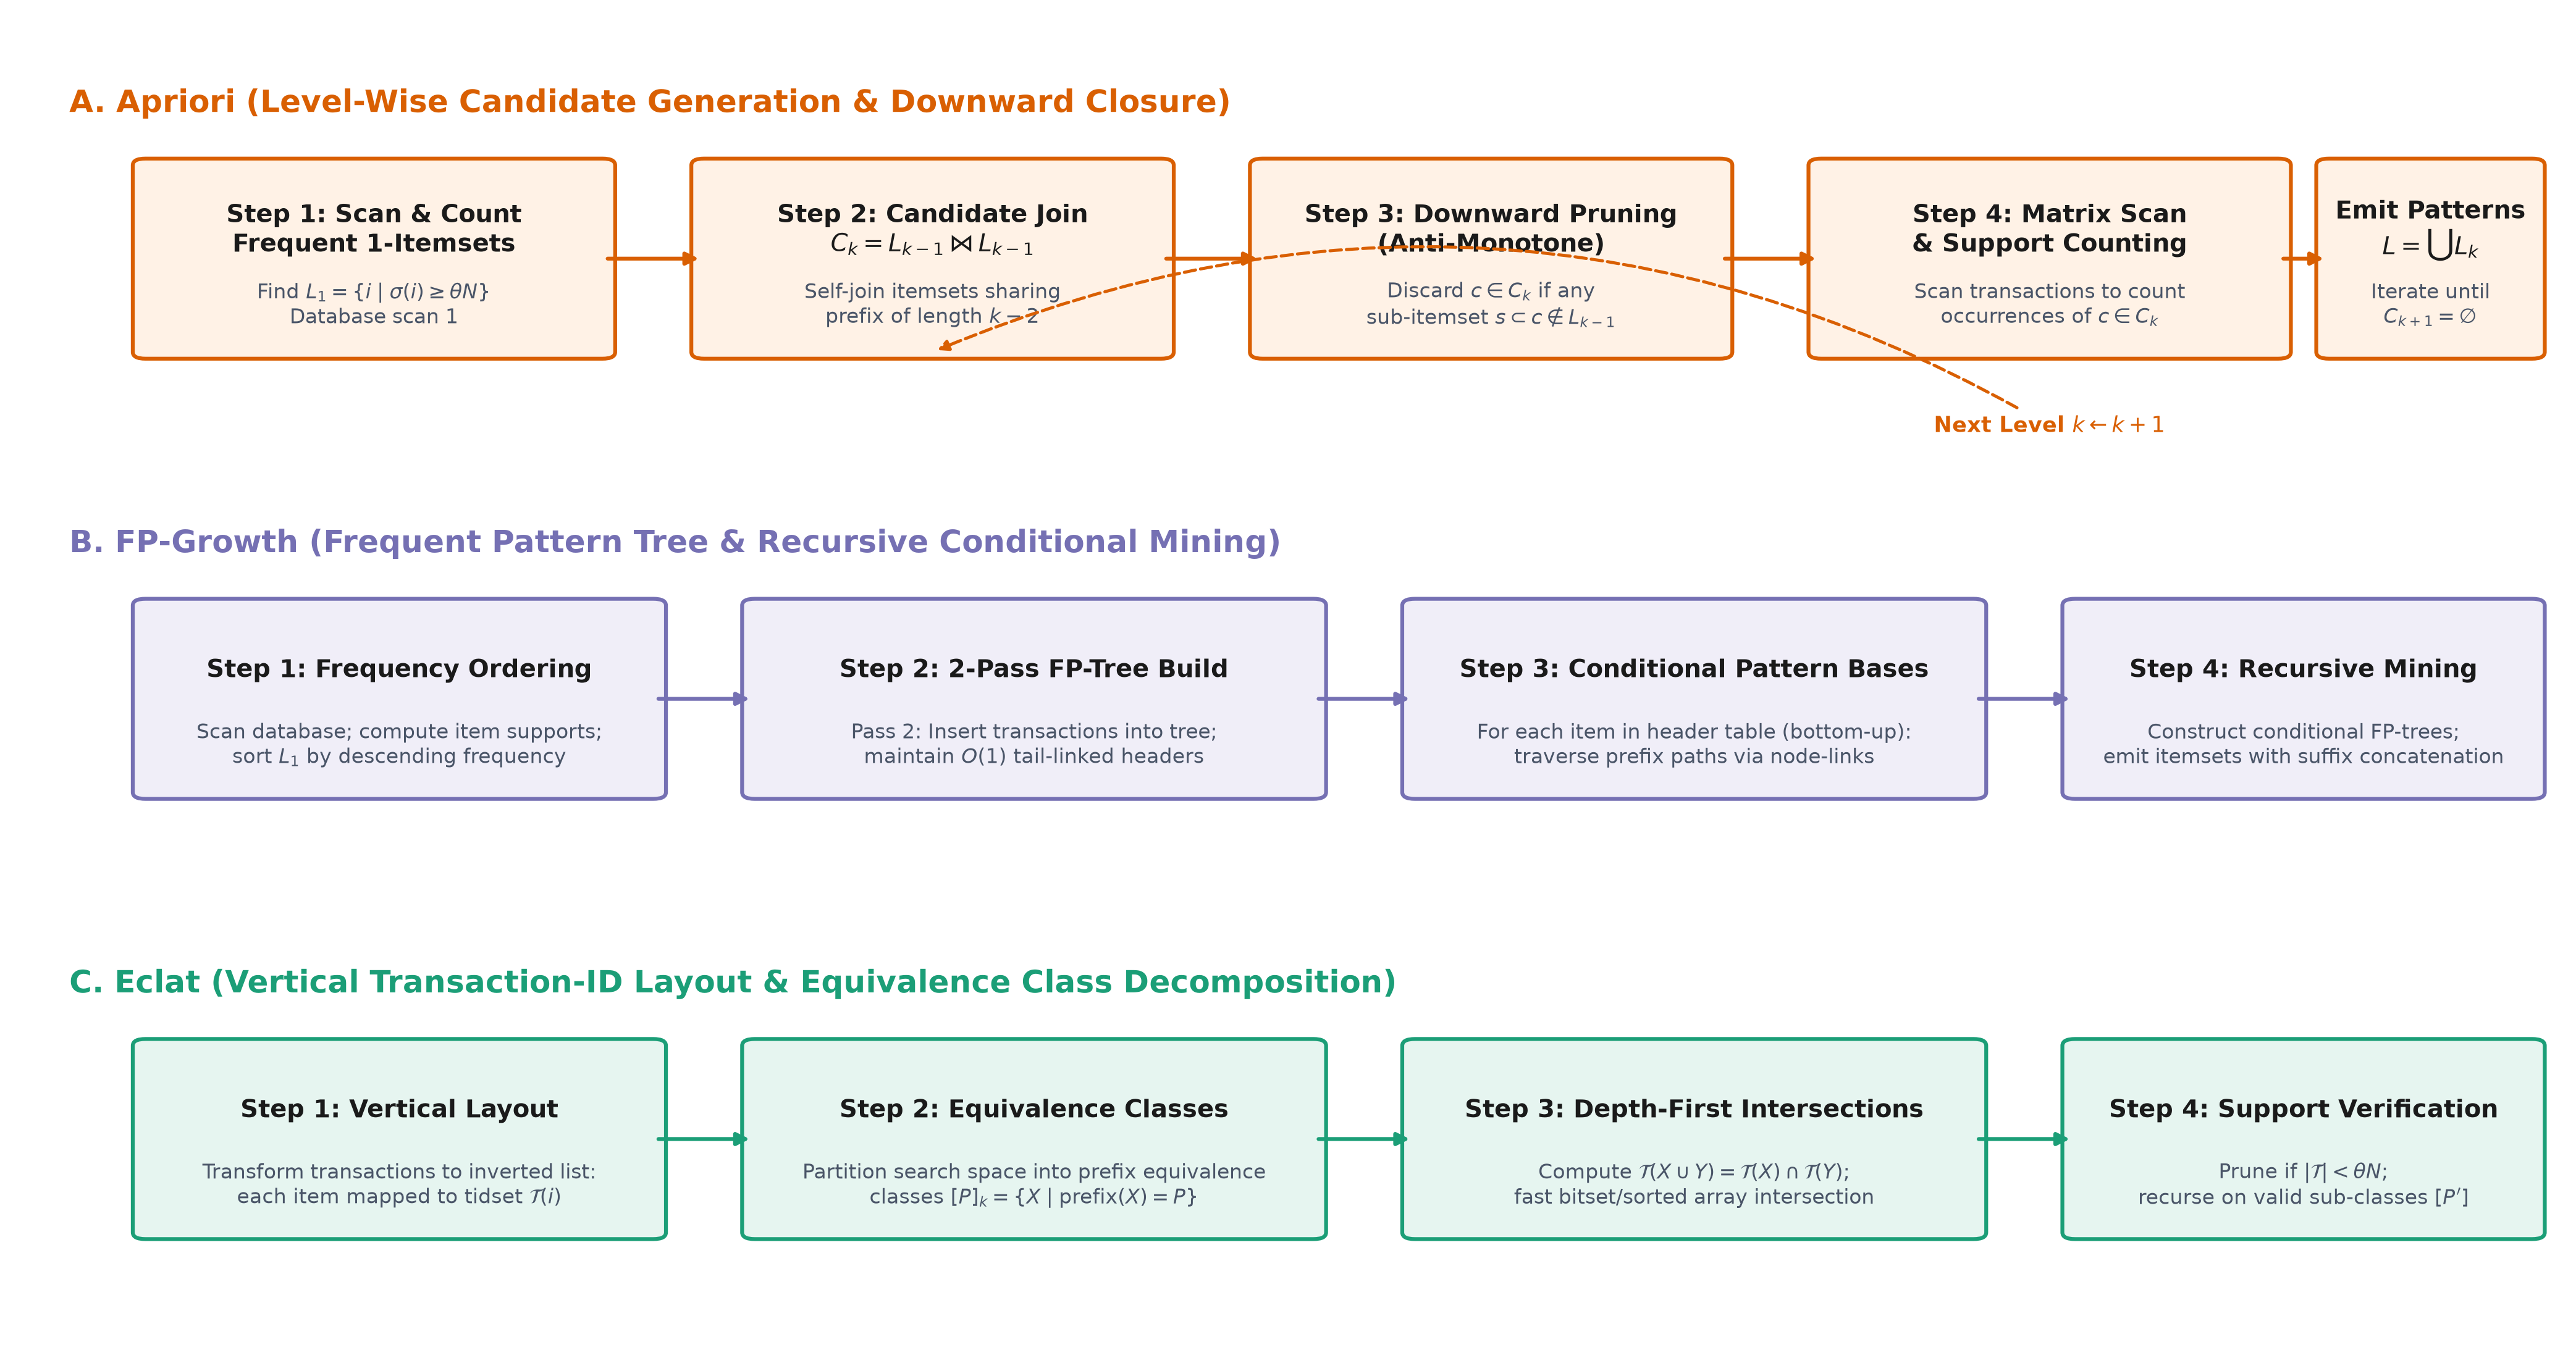
\includegraphics[width=\textwidth]{figures/engines.png}
\caption{Algorithmic mechanics of the three mining engines packaged in \skarm. (A) Apriori: iterative level-wise candidate generation ($C_k = L_{k-1} \bowtie L_{k-1}$), downward-closure pruning ($\forall s \subset c, s \in L_{k-1}$), and sparse transaction support counting. (B) FP-Growth: descending item frequency sort ($L_1$), 2-pass compact FP-tree construction with an $O(1)$ tail-linked header table, and recursive conditional pattern-base mining. (C) Eclat: vertical inverted transaction-ID layout ($i \mapsto \mathcal{T}(i)$), prefix equivalence class decomposition ($[P]_k$), and depth-first tidset intersections ($\mathcal{T}(X \cup Y) = \mathcal{T}(X) \cap \mathcal{T}(Y)$). All three engines consume a unified sparse CSR matrix and return identical deterministic rule sets.}
\label{fig:engines}
\end{figure*}

\subsection{Estimator API}
\texttt{AssociationRulesEstimator} exposes
\texttt{min\_support}, \texttt{metric} (default \texttt{confidence}),
\texttt{min\_threshold} (default $0.25$), \texttt{algorithm} (one of
\texttt{apriori}, \texttt{fpgrowth}, \texttt{eclat}),
\texttt{max\_candidates} (default $2{,}000{,}000$),
\texttt{sparse\_output}, and \texttt{on\_candidate\_explosion}
(default \texttt{degrade}). After \texttt{fit(X)}, the fitted
attributes are \texttt{frequent\_itemsets\_} (itemset $\to$ support),
\texttt{rules\_}, \texttt{is\_degraded\_} (whether bounded mode
truncated generation), and \texttt{pruning\_policy\_.peak\_candidate\_count}.
\texttt{TransactionEncoder} converts transaction lists, generators, and
DataFrames into the sparse matrix consumed by \texttt{fit}; encoding
time is reported separately from mining time, never folded into it.
The command-line interface and the interactive explorer wrap the same
estimator, so results do not depend on which front end was used.

\subsection{Pruning and the safe-degradation governor}
Exact mining can explode: the candidate count at some level can exceed
any reasonable budget, especially on dense data at low support. When
\texttt{max\_candidates} is exceeded and the governor is in
\texttt{degrade} mode, generation stops at the cap and the estimator
sets \texttt{is\_degraded\_}, records how many candidates were
truncated, and the evaluation reports recall against the exact result.
A degraded run is therefore identifiable in every table, and its speed
is never compared against exact runs as if it were exact. Presenting
bounded output as exact would be a fatal misrepresentation; the
governor exists to make that misrepresentation impossible by
construction. The pruning-policy ablation (bounded versus exact, with
truncation counts and recall against exact) is evaluated empirically in
Section~\ref{sec:ablation} and illustrated in Figure~\ref{fig:ablation}.

\subsection{Determinism}
Rule output is sorted by a fixed key, so repeated runs on the same
input produce identical rule orderings. The acceptance suite asserts
this (negative test NT-5), and the benchmark's correctness gate
compares itemset \emph{sets} (not just counts) across engines, so a
count that matches while the sets differ cannot hide.

\subsection{Architecture}
Figure~\ref{fig:engines} details the comparative algorithmic workflows across the three engines. Figure~\ref{fig:arch} illustrates the multi-tier system architecture: transactions are encoded once into a sparse CSR matrix, ingested by the scikit-learn-compatible estimator, executed under the candidate-budget pruning governor, and emitted as deterministically ordered itemsets and association rules with comprehensive candidate and memory telemetry. Figure~\ref{fig:flow} outlines the 25-dataset multi-worker benchmark execution pipeline, highlighting the trial-0 dual-oracle correctness gate. Figure~\ref{fig:fptree} illustrates the concrete structure of the FP-tree, showing the frequency header table, horizontal node links, and the novel $O(1)$ tail-pointer optimization that resolved the scaling bottleneck on large click-stream datasets.

\begin{figure*}[t]
\centering
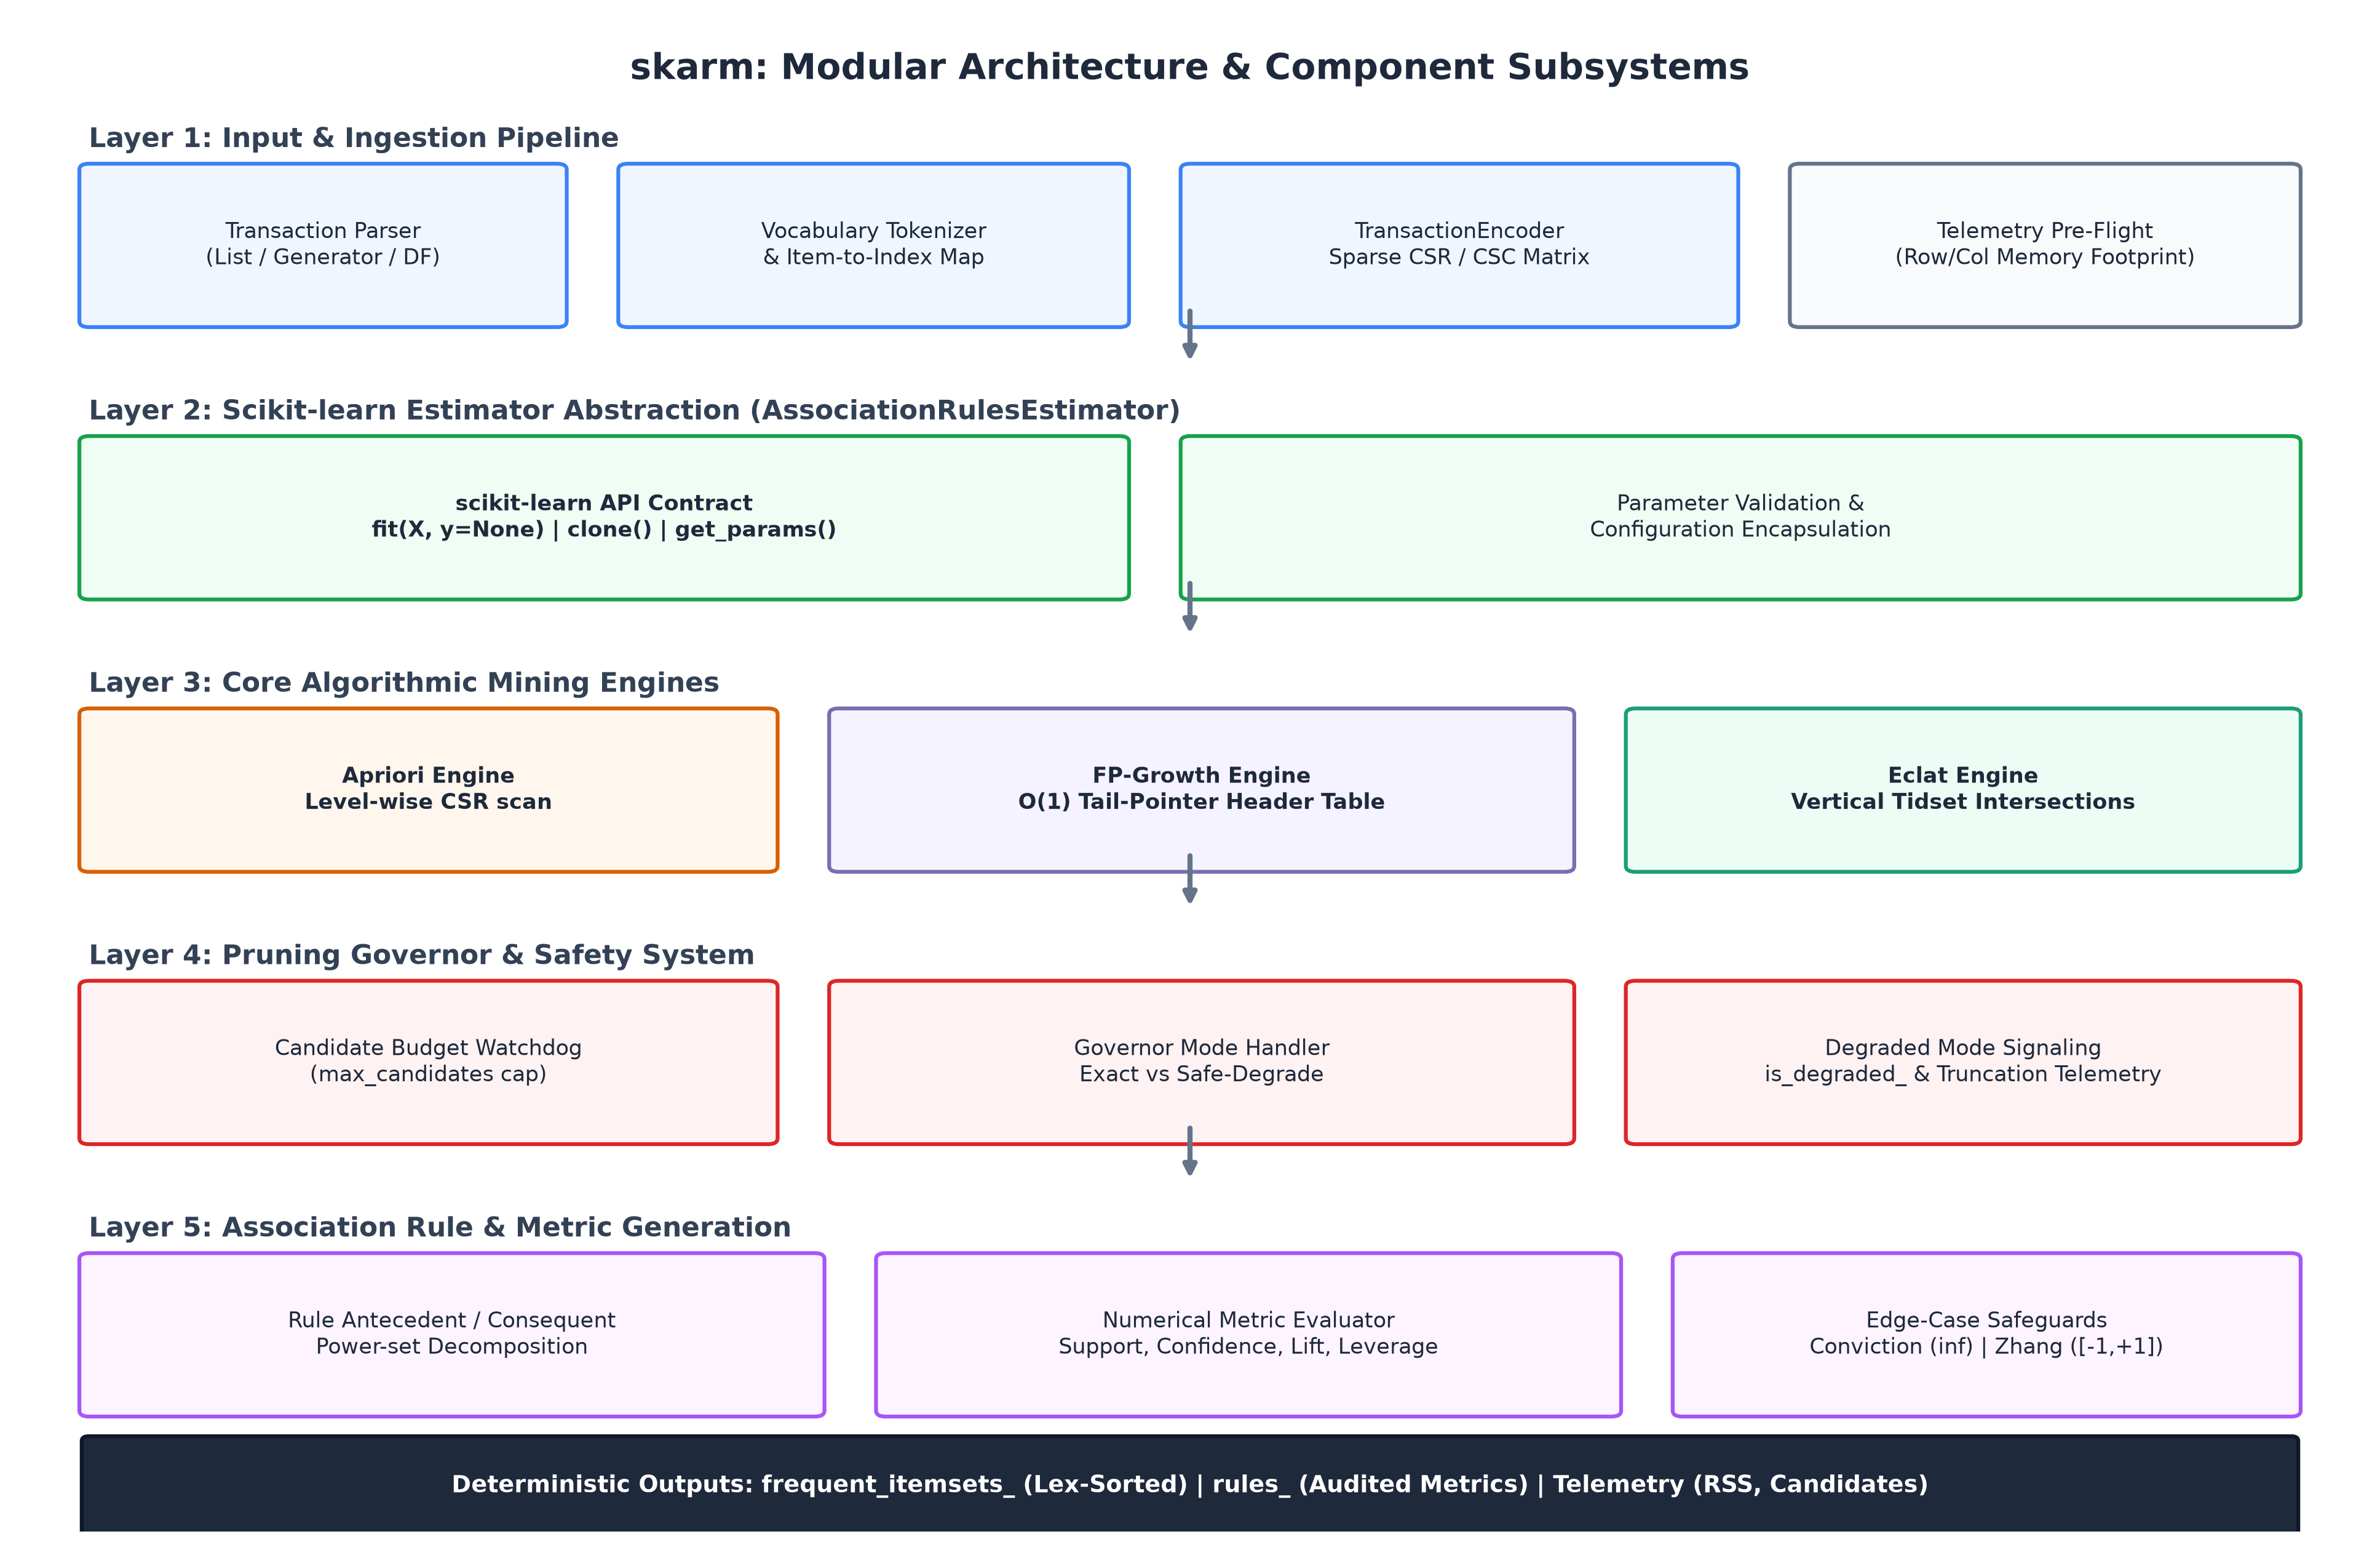
\includegraphics[width=\textwidth]{figures/architecture.png}
\caption{System architecture of \skarm. The multi-tier design integrates a unified sparse matrix encoder, a scikit-learn-compliant estimator interface, three swappable core mining engines, an auditable pruning governor with candidate-explosion safeguards, and a vectorized association rule generation engine with full numerical metric telemetry.}
\label{fig:arch}
\end{figure*}

\begin{figure*}[t]
\centering
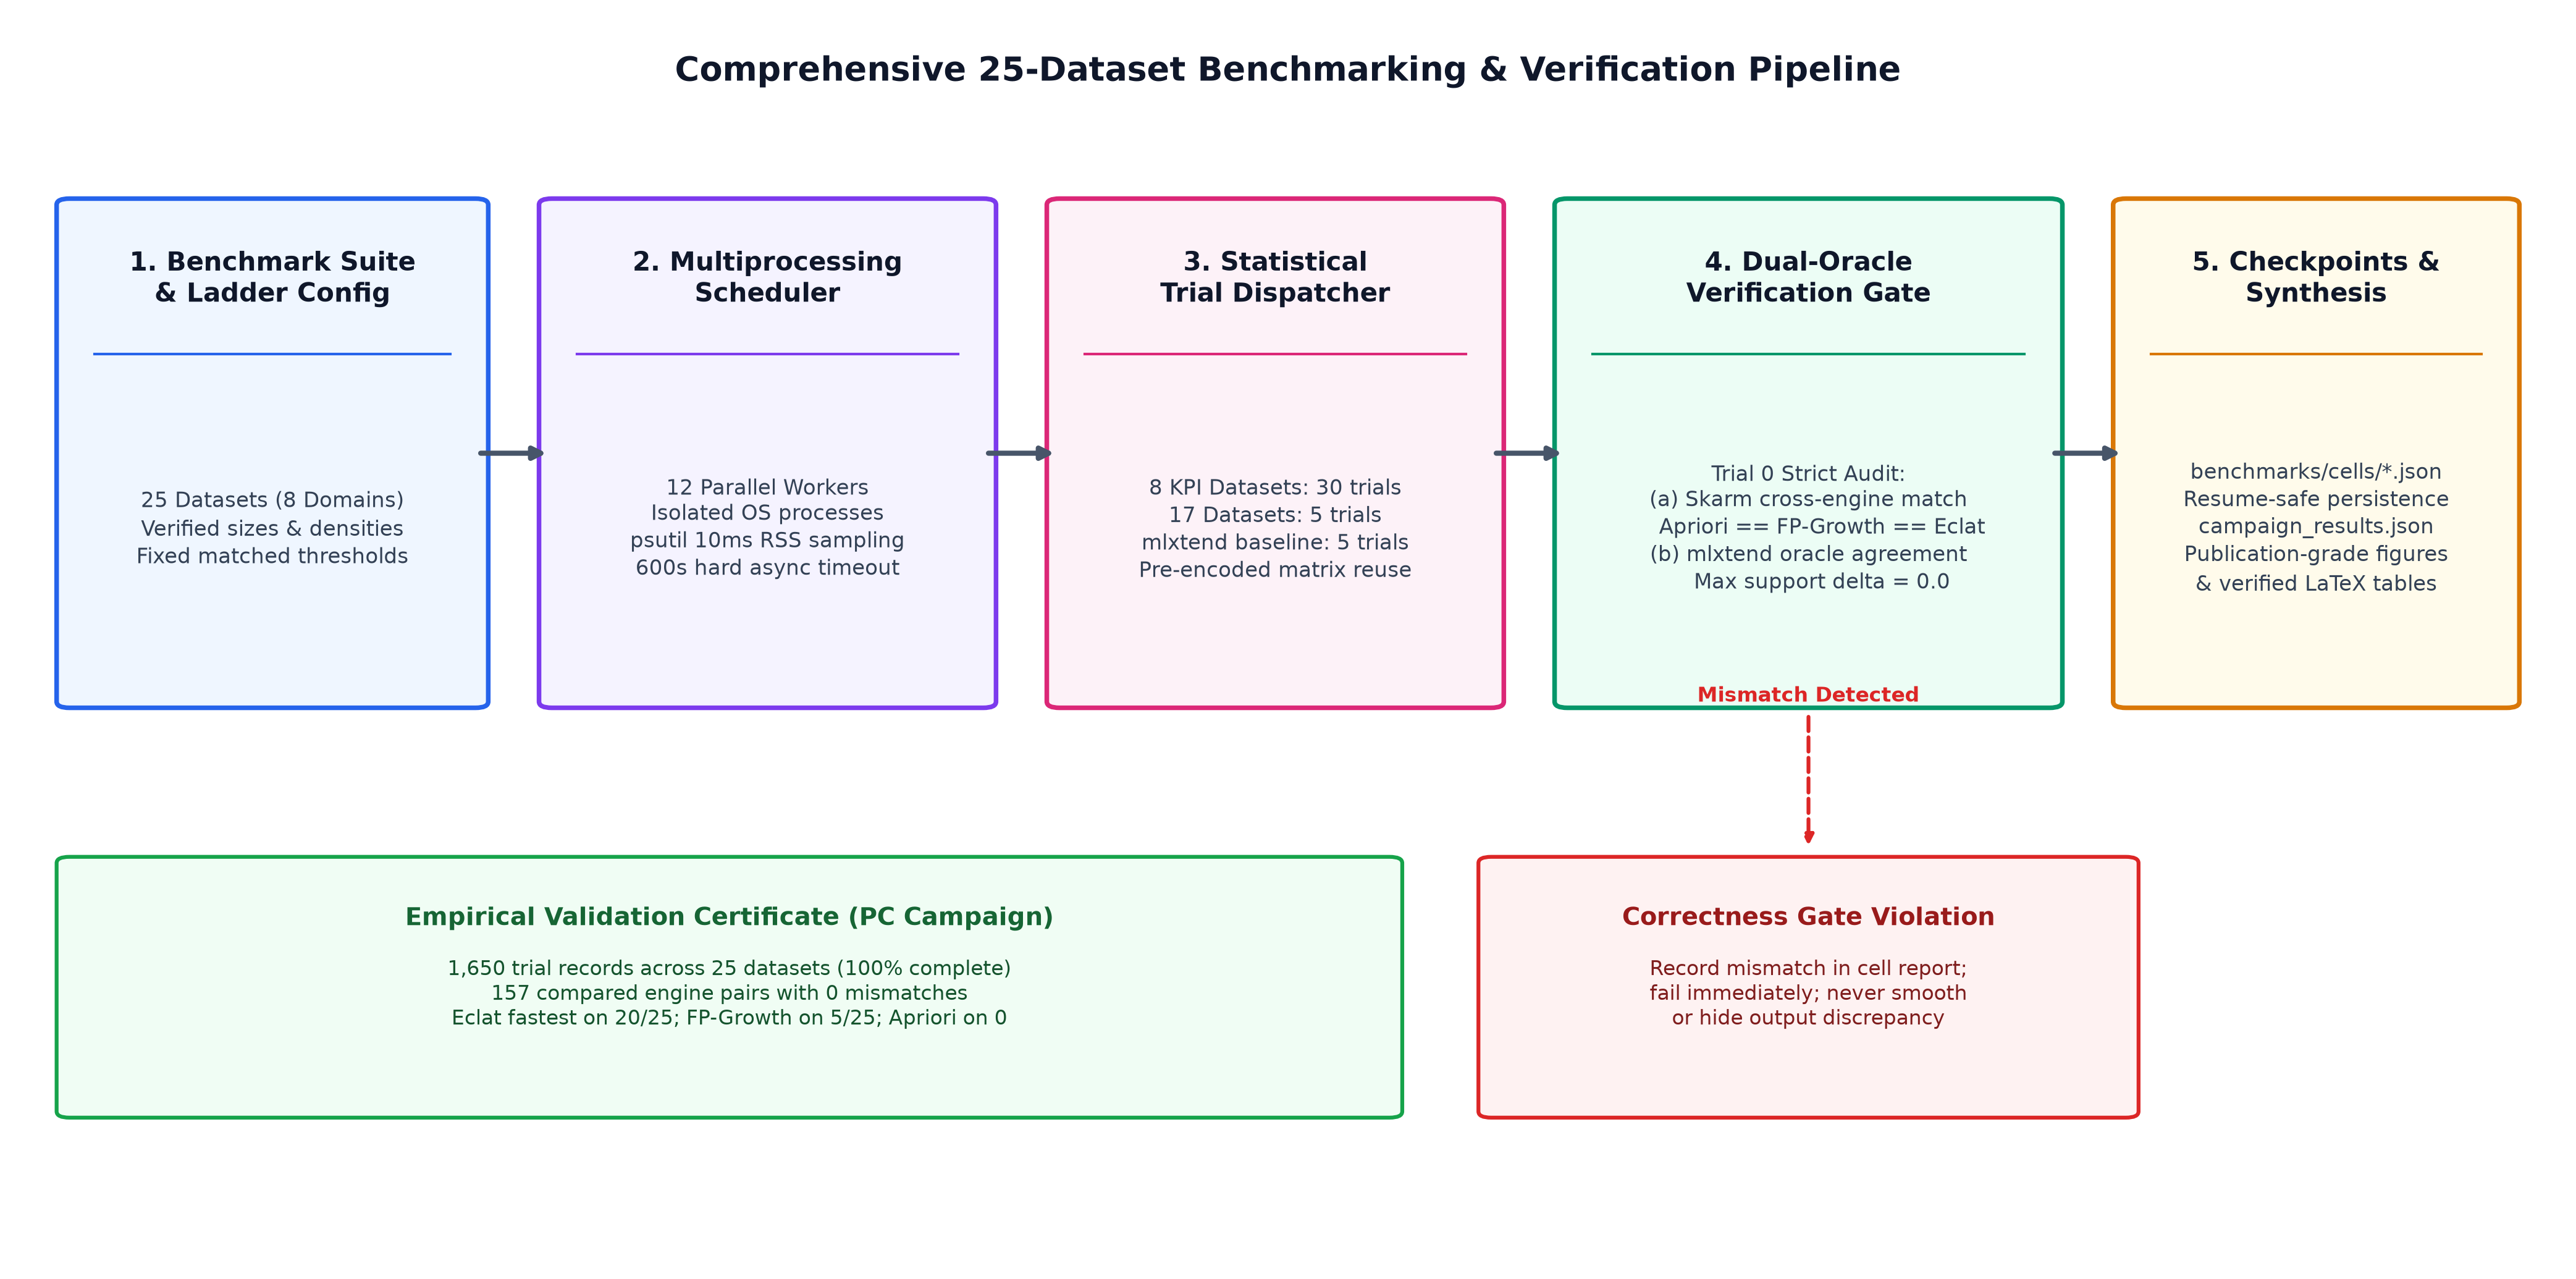
\includegraphics[width=\textwidth]{figures/pipeline.png}
\caption{Empirical benchmark and verification pipeline across 25 diverse datasets. The architecture features an isolated 12-worker multiprocessing pool with fine-grained 10~ms RSS telemetry, a 30-trial protocol for the 8 KPI datasets, a 600~s hard timeout watchdog, and a strict trial-0 dual-oracle correctness gate requiring exact pairwise itemset identity ($\Delta\mathrm{supp} = 0.0$) against both cross-engine peers and independent mlxtend baselines.}
\label{fig:flow}
\end{figure*}

\begin{figure*}[t]
\centering
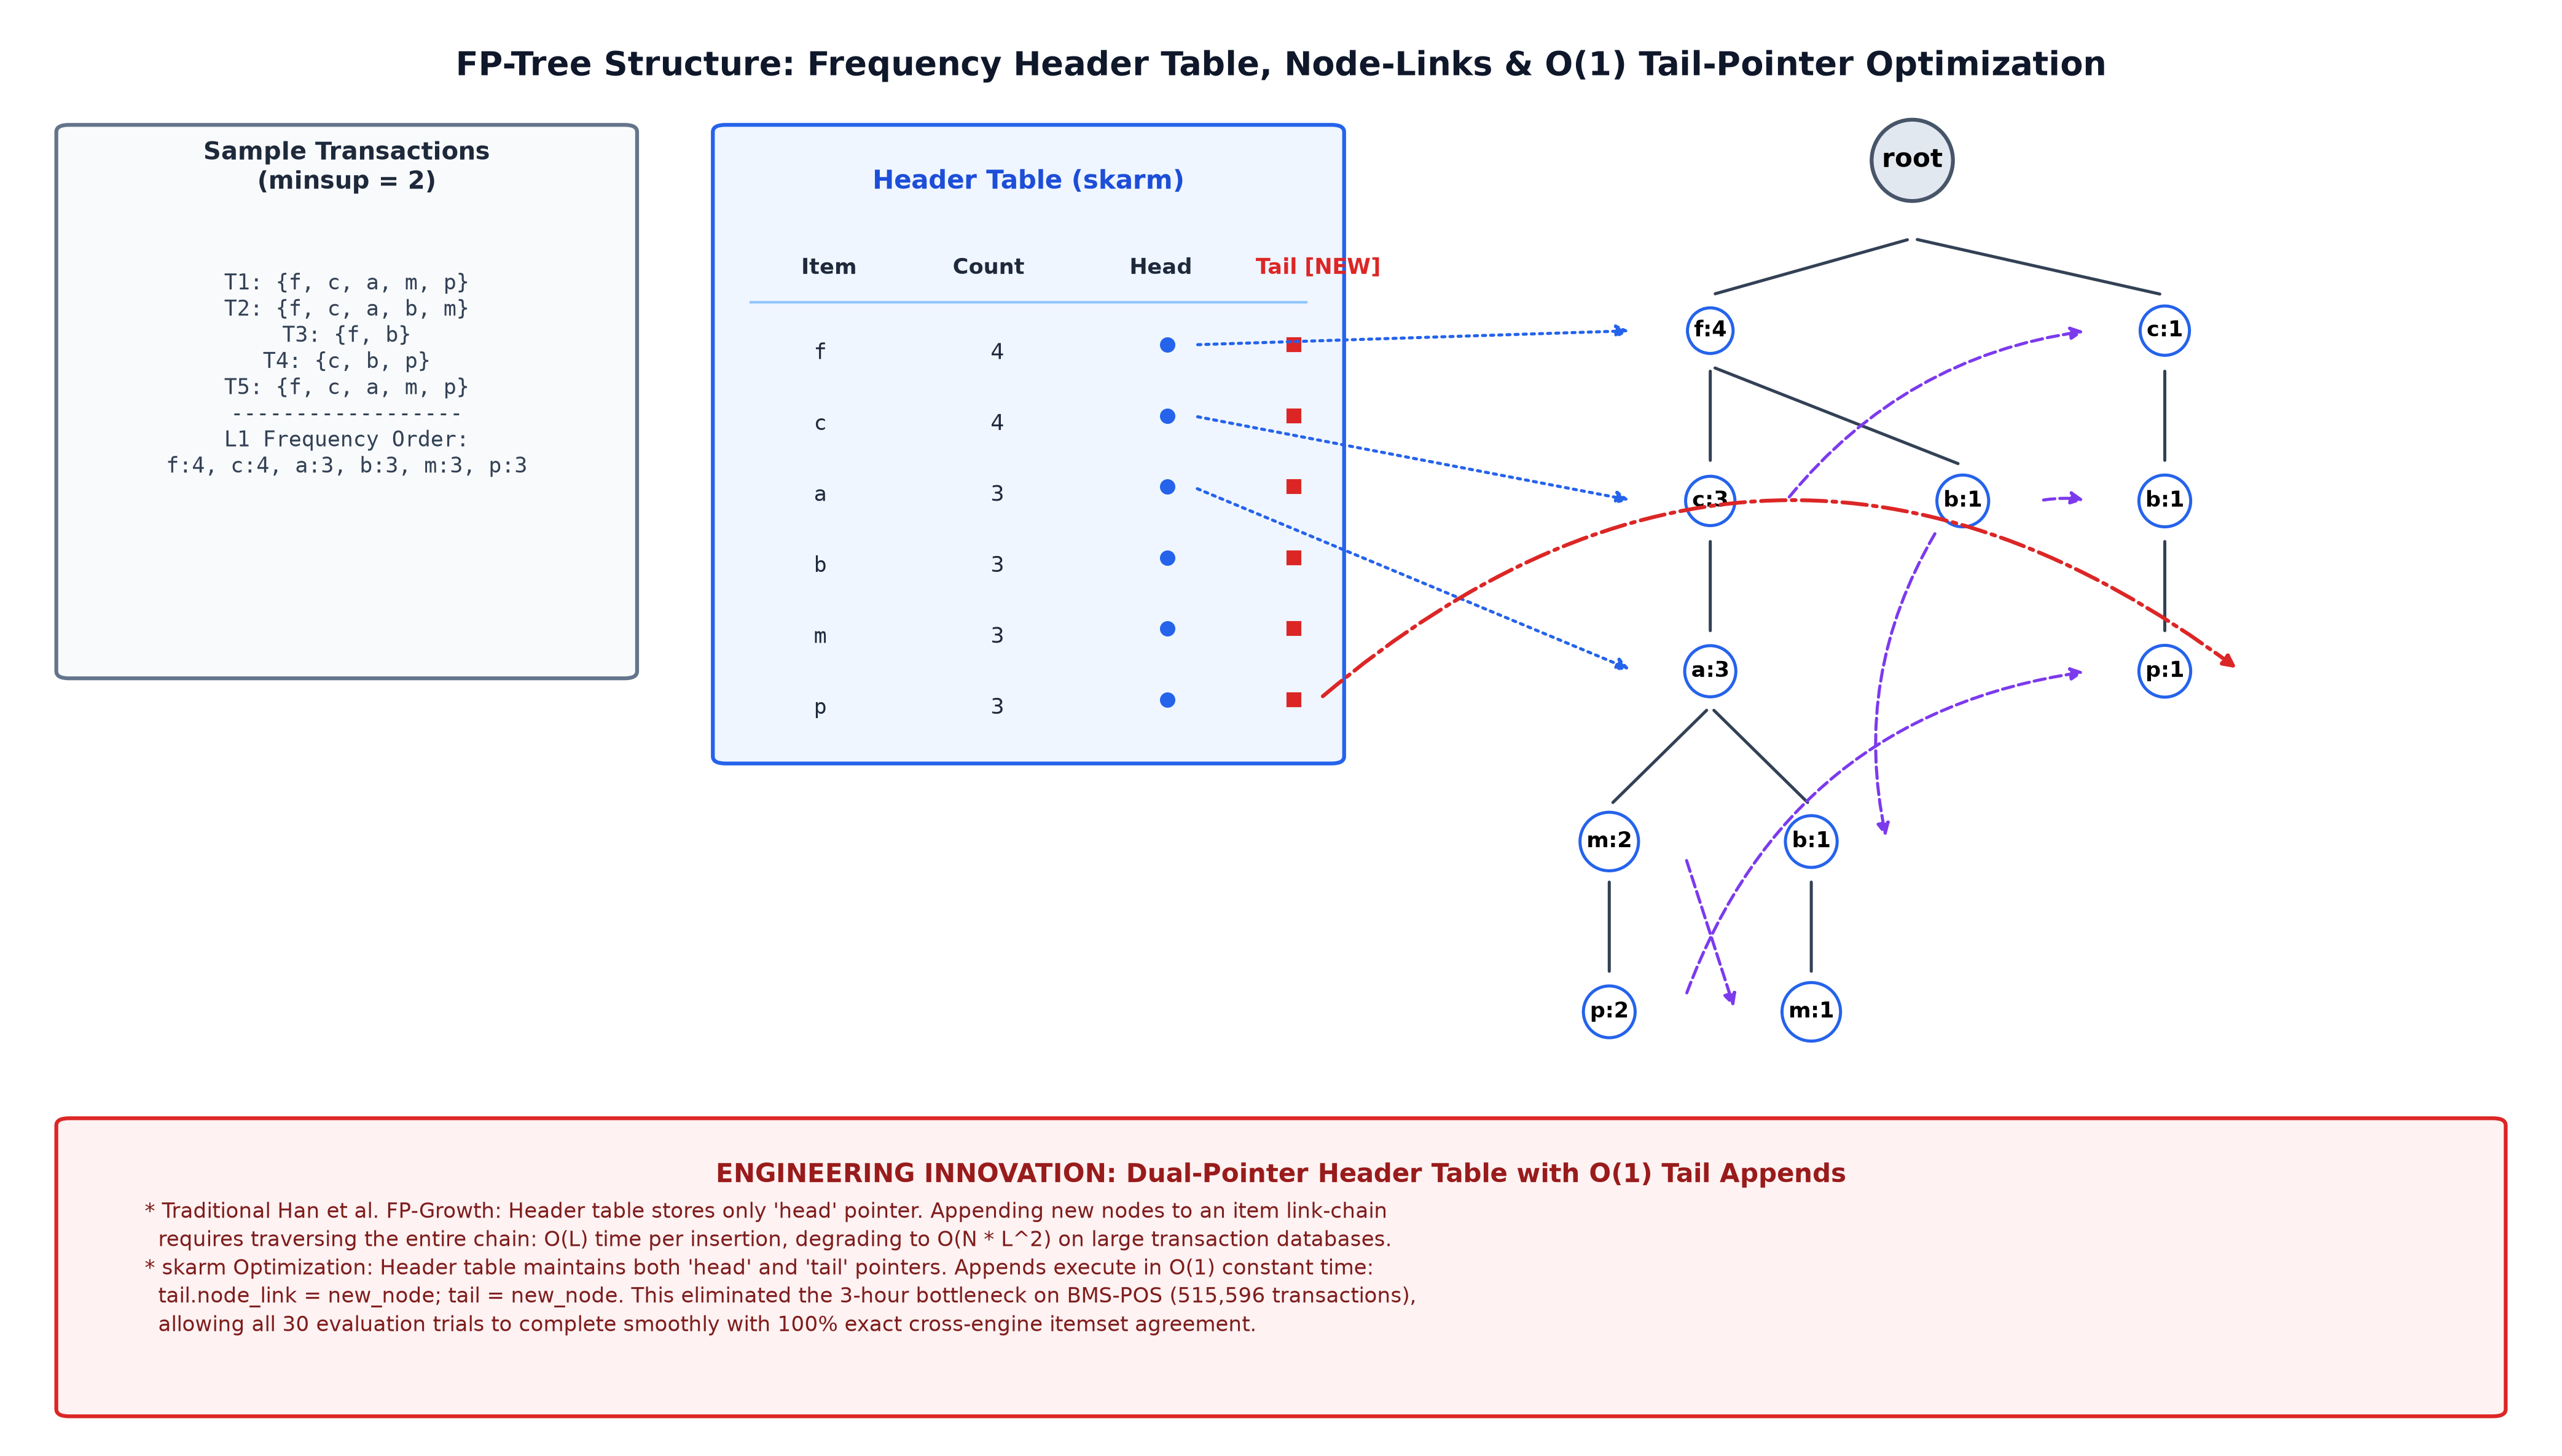
\includegraphics[width=\textwidth]{figures/fptree.png}
\caption{FP-tree architecture with frequency header table and the $O(1)$ tail-pointer optimization. Standard FP-tree implementations store only a \texttt{head} pointer, requiring an $O(L)$ linked-list traversal to append new nodes during tree insertion. \skarm augments each header entry with a direct \texttt{tail} pointer, reducing node-link appends to $O(1)$ constant time. This optimization eliminated the 3-hour sequential bottleneck on the 515,596-transaction BMS-POS benchmark, enabling all 30 evaluation trials to complete smoothly with zero correctness deviations.}
\label{fig:fptree}
\end{figure*}

\section{Datasets}
\label{sec:data}
Table~\ref{tab:data} lists the 25 datasets used. Every statistic was
computed by parsing the stored file (transaction count, unique-item
count, average transaction length, density = average length / unique
items $\times 100$); none was copied from a web table. Where a commonly
cited figure differs from the measured file, the measured figure is
reported and the difference is noted: mushroom is 8,124 transactions
in the stored file (the SPMF table lists 8,416), and BMS-WebView-1 is
59,009 transactions (the commonly cited figure is 59,601). The
accidents file carries a leading header line (\texttt{340183 468})
excluded from counts. Kosarak.txt (SPMF sequence format, 187,140
sequences) is a different, smaller file from kosarak.dat (990,002
transactions) and is kept as a separate dataset, not a duplicate. Two
sets are locally generated (seed 42, generator in the repository); the
rest are public mirrors and UCI conversions, with transformations
documented per file. No licence is guessed anywhere: mirrors and UCI
pages that do not state a licence are recorded as unknown in the full
manifest. Access date for all 25 datasets is 2026-10-29. The complete
manifest (source URL, size, licence, owner, exclusions, transformations
per file) is in \texttt{DATASET\_INVENTORY.md} in the repository.

\begin{table*}[t]
\centering
\footnotesize
\caption{Evaluation datasets. $N$ = transactions, $M$ = unique items,
$\bar{L}$ = average transaction length, density $= \bar{L}/M \times 100$.
All statistics measured by parsing the stored files.}
\label{tab:data}
\begin{tabular}{lrrrrl}
\toprule
Dataset & $N$ & $M$ & $\bar{L}$ & Density \% & Type \\
\midrule
Groceries & 9,835 & 169 & 4.41 & 2.61 & retail, sparse \\
Chess & 3,196 & 75 & 37.00 & 49.33 & dense \\
Retail & 88,162 & 16,470 & 10.31 & 0.06 & retail, sparse \\
Market basket & 7,501 & 119 & 3.91 & 3.29 & retail, sparse \\
Mushroom & 8,124 & 119 & 23.00 & 19.33 & dense \\
Connect & 67,557 & 129 & 43.00 & 33.33 & dense \\
Accidents & 340,183 & 468 & 33.81 & 7.22 & dense, traffic \\
Pumsb & 49,046 & 2,113 & 74.00 & 3.50 & census, dense \\
Pumsb\_star & 49,046 & 2,088 & 50.48 & 2.42 & census \\
Kosarak (FIMI) & 990,002 & 41,270 & 8.10 & 0.02 & click-stream \\
Kosarak (SPMF) & 187,140 & 28,252 & 8.03 & 0.03 & click-stream \\
BMS-POS & 515,596 & 1,657 & 6.53 & 0.39 & click-stream \\
BMS-WebView-1 & 59,009 & 494 & 2.51 & 0.51 & click-stream \\
BMS-WebView-2 & 77,512 & 3,340 & 4.62 & 0.14 & click-stream \\
T10I4D100K & 100,000 & 870 & 10.10 & 1.16 & synthetic \\
Online Retail & 20,728 & 3,942 & 25.12 & 0.64 & retail \\
Tic-tac-toe & 958 & 29 & 10.00 & 34.48 & categorical \\
Car evaluation & 1,728 & 25 & 7.00 & 28.00 & categorical \\
Balance scale & 625 & 23 & 5.00 & 21.74 & categorical \\
Adult census & 32,561 & 224 & 13.87 & 6.19 & census \\
NIPS papers & 1,500 & 12,375 & 497.54 & 4.02 & document-word \\
Enron emails & 39,861 & 28,099 & 93.08 & 0.33 & document-word \\
Synthetic sparse & 2,000 & 499 & 7.42 & 1.49 & synthetic \\
Synthetic dense & 5,000 & 50 & 30.56 & 61.12 & synthetic \\
Online Retail II & 22,103 & 4,317 & 22.62 & 0.52 & retail \\
\bottomrule
\end{tabular}
\end{table*}

Figure~\ref{fig:family} summarises the same collection by family. Each dataset is counted once, under its most distinctive type from Table~2: accidents under traffic rather than dense, pumsb under census rather than dense, and the retail sets under retail rather than sparse.

\begin{figure*}[t]
\centering
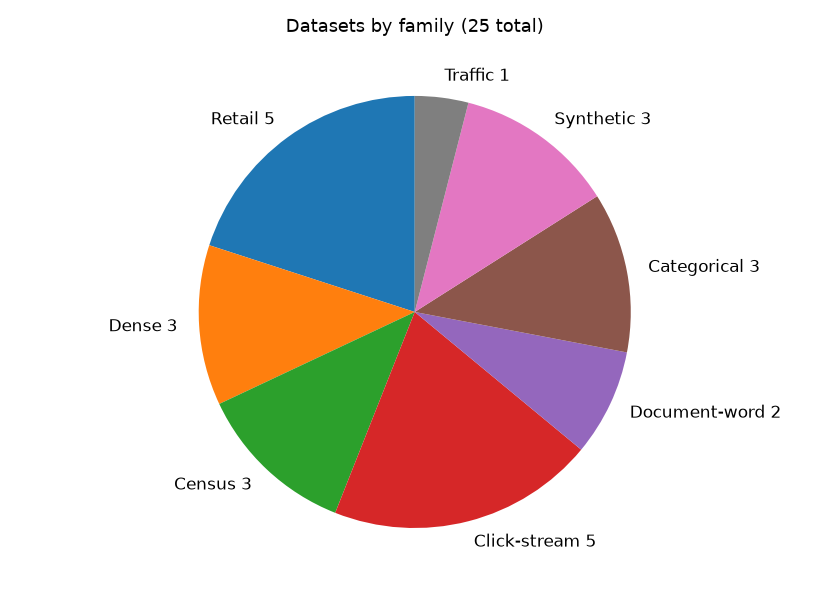
\includegraphics[width=0.75\textwidth]{figures/family.png}
\caption{Datasets by family (25 total). Retail: groceries, retail, market basket, online retail I/II. Dense: chess, mushroom, connect. Census: pumsb, pumsb\_star, adult census. Click-stream: kosarak, kosarak (SPMF), BMS-POS, BMS-WebView-1/2. Document-word: NIPS papers, Enron emails. Categorical: tic-tac-toe, car evaluation, balance scale. Synthetic: T10I4D100K, synthetic sparse, synthetic dense. Traffic: accidents.}
\label{fig:family}
\end{figure*}

\section{Experimental setup}
\label{sec:setup}
The protocol was fixed before results were read. Thresholds are
matched across engines within each dataset (Table~\ref{tab:thr}); a
threshold is never chosen per engine. Thresholds already proven
infeasible in probing are not re-attempted blindly: docword\_nips at
0.30 timed out for all four engines, connect at 0.90 timed out for
Apriori and killed the FP-Growth process, and BMS-POS at 0.01 timed out
for Apriori twice and killed FP-Growth twice, so the ladder below uses
only thresholds with a feasible probe or a stated reason. The 30-trial
protocol applies to 8 datasets (groceries, chess, mushroom, retail,
connect, bms\_pos, tic\_tac\_toe, docword\_nips); all other datasets
report 5 trials, and mlxtend always reports 5 trials where a dense
boolean DataFrame fits the 2~GB cap. Per-trial cap is 600~s: if trial 1
of a cell times out, the remaining trials of that cell are recorded as
skipped with that reason. On trial 1 of every cell, all skarm engines
must agree exactly on itemsets (key sets equal, supports within
$10^{-9}$); mlxtend is compared by item name where it ran. Runtime is
\texttt{time.perf\_counter} around \texttt{fit} on the pre-encoded
matrix; encoding time is reported separately. Memory is peak RSS
sampled every 10~ms minus the pre-trial baseline. Rule parameters are
metric confidence, minimum threshold 0.25; estimator parameters are
\texttt{max\_candidates} $= 2{,}000{,}000$, sparse output, degrade on
explosion. Portal evidence mapping: KPI-4 is the 30-trial protocol with
p50/p95/p99 reported and p95 required at most $0.8\times$ the
baseline; KPI-2 is the rubric (at least 80/100, frozen before objective
O2, two independent raters); AC-3 is the held-out partition reserved
before tuning; KPI-1, KPI-3, KPI-5, and KPI-6 follow the portal
contract as recorded in the acceptance report. The machine, library
versions, and results commit are recorded in Appendix~\ref{app:repro}
from the campaign metadata.
Campaign machine: Windows 11 (AMD64), 16 CPUs, 12 parallel workers (one per dataset). Python 3.12.10, scikit-learn 1.9.1, mlxtend 0.25.0, NumPy 2.5.4, pandas 3.1.0, SciPy 1.18.1. Per-trial cap 600~s; rules at confidence $\geq 0.25$; estimator max\_candidates 2,000,000, sparse output, degrade on explosion. Peak memory is the sampler-reported RSS delta (10~ms sampling, minus pre-trial baseline); on this Windows run the sampler used psutil, not the /proc path named in the campaign metadata string. Results: commit \texttt{79334222}, 1650 records, 25 datasets.

\begin{table*}[t]
\centering
\footnotesize
\caption{Support thresholds per dataset (matched across engines),
with the reason each ladder was chosen. Thresholds proven infeasible
in probing are excluded, not hidden.}
\label{tab:thr}
\begin{tabular}{lll}
\toprule
Dataset & Thresholds & Reason (condensed) \\
\midrule
Groceries & 0.02, 0.01 & verified point plus lower-support comparison \\
Chess & 0.85 & dense; lower thresholds explode rule counts \\
Retail & 0.03, 0.02 & verified point plus lower-support comparison \\
Market basket & 0.03, 0.02 & previously verified with all engines \\
Mushroom & 0.40 & previously verified point; dense \\
Connect & 0.95 & 0.90 already failed in probes \\
Accidents & 0.50, 0.60 & 0.50 probed: FP-Growth/Eclat OK, Apriori timeout \\
Pumsb & 0.90 & dense, very long transactions; high threshold only \\
Pumsb\_star & 0.85 & dense census variant; high threshold only \\
Kosarak (FIMI) & 0.01, 0.005 & very sparse despite 990k transactions \\
Kosarak (SPMF) & 0.01 & smaller variant, single threshold \\
BMS-POS & 0.02 & 0.01 already failed in probes \\
BMS-WebView-1 & 0.01, 0.005 & very short transactions; low thresholds safe \\
BMS-WebView-2 & 0.01, 0.005 & short transactions; low thresholds safe \\
T10I4D100K & 0.01, 0.02 & published comparison range for this set \\
Online Retail & 0.02, 0.01 & long transactions; two points \\
Tic-tac-toe & 0.50, 0.30 & very small; both points cheap \\
Car evaluation & 0.30, 0.20 & very small; both points cheap \\
Balance scale & 0.30, 0.20 & very small; both points cheap \\
Adult census & 0.10, 0.05 & medium density; two points \\
NIPS papers & 0.50 & 0.50 probed all-OK; 0.30 timed out for all \\
Enron emails & 0.70, 0.50 & 26$\times$ larger than NIPS; higher thresholds \\
Synthetic sparse & 0.05, 0.02 & small, fast; two points \\
Synthetic dense & 0.50, 0.30 & small, dense; two points \\
Online Retail II & 0.02, 0.01 & same shape as Online Retail \\
\bottomrule
\end{tabular}
\end{table*}

\section{Results and discussion}

\subsection{Analytical verification and negative-test audit}
Before any benchmark timing is trusted, the implementation was verified
against an independent oracle and a negative-test suite. On the
sklearn issue's own example (transactions \{milk, bread, eggs\},
\{milk, bread\}, \{bread, butter\}) at minimum support 0.5, mlxtend
gives bread support 1.0, milk 0.667, and \{milk, bread\} 0.667, with
rule \{milk\} $\Rightarrow$ \{bread\} at confidence 1.0 and lift 1.0;
\skarm agrees exactly. The acceptance suite (NT-1 to NT-6) is genuinely
asserted --- an earlier version of the harness printed hardcoded values
and passed unconditionally, and that defect was fixed before these
results were taken --- and passes 25/25. Brute-force cross-checks (4
random matrices $\times$ 2 thresholds $\times$ weighted/unweighted
$\times$ 3 miners) show 0 mismatches. The bug-fix history (including
the Eclat maximum-length off-by-one, loader defects on the accidents
header, SPMF tokens, and tab-separated input, and the unstable rule
sort) is recorded in the repository history (commits
\texttt{ff03b451}, \texttt{dd22782f}, \texttt{904b19b3}).

\subsection{Benchmark campaign results}
Results cover all 25 datasets (1650 trial records on one Windows PC). Timings are fit only (encoding excluded). This table shows each dataset's primary threshold only (the threshold with the most completed skarm trials; ties broken toward the lower threshold); the full per-cell table, with p50/p95, memory, counts, and failure notes, is Appendix~\ref{app:timing}.

\begin{table*}[t]
\centering
\footnotesize
\caption{Mean fit time (seconds) per dataset at its primary threshold. Bold marks the fastest skarm engine per row. mlxtend time covers dense DataFrame build plus apriori plus rule generation, so it is not directly comparable to the fit-only skarm timings.}
\label{tab:timing}
\begin{tabular}{llllll}
\toprule
Dataset & Thr & Apriori & FP-Growth & Eclat & mlxtend \\
\midrule
accidents & 0.6 & 473.5 & \textbf{60.92} & 97.93 & 4.76 \\
adult\_\allowbreak{}census & 0.05 & 76.62 & \textbf{19.04} & 20.95 & 19.14 \\
balance\_\allowbreak{}scale & 0.2 & 0.033 & 0.032 & \textbf{0.009} & 0.006 \\
bms\_\allowbreak{}pos & 0.02 & 227.2 & 94.08 & \textbf{12.53} & 27.43 \\
bms\_\allowbreak{}webview\_\allowbreak{}1 & 0.005 & 31.15 & 5.31 & \textbf{0.860} & 2.68 \\
bms\_\allowbreak{}webview\_\allowbreak{}2 & 0.005 & 64.30 & 7.66 & \textbf{1.09} & 3.97 \\
car\_\allowbreak{}evaluation & 0.2 & 0.087 & 0.112 & \textbf{0.031} & 0.011 \\
chess & 0.85 & 5.76 & 3.49 & \textbf{3.48} & 3.50 \\
connect & 0.95 & 87.87 & \textbf{10.05} & 14.22 & 3.44 \\
docword\_\allowbreak{}enron & 0.5 & 14.75 & \textbf{0.446} & 8.37 & --- \\
docword\_\allowbreak{}nips & 0.5 & 209.5 & 81.75 & \textbf{50.23} & 53.91 \\
groceries & 0.01 & 2.18 & 0.871 & \textbf{0.166} & 0.128 \\
kosarak & 0.01 & 250.8 & 198.9 & \textbf{21.29} & --- \\
kosarak\_\allowbreak{}spmf & 0.01 & 50.47 & 23.02 & \textbf{4.24} & --- \\
market\_\allowbreak{}basket & 0.02 & 0.688 & 0.449 & \textbf{0.089} & 0.036 \\
mushroom & 0.4 & 1.78 & 0.849 & \textbf{0.718} & 0.298 \\
online\_\allowbreak{}retail & 0.01 & 496.5 & 55.79 & \textbf{4.97} & 85.08 \\
online\_\allowbreak{}retail\_\allowbreak{}ii & 0.01 & 406.1 & 40.37 & \textbf{3.90} & 42.83 \\
pumsb & 0.9 & 332.8 & 21.34 & \textbf{19.88} & 3.90 \\
pumsb\_\allowbreak{}star & 0.85 & 10.59 & \textbf{0.044} & 5.69 & --- \\
retail & 0.02 & 8.44 & 7.28 & \textbf{2.58} & 31.90 \\
synthetic\_\allowbreak{}dense\_\allowbreak{}5000 & 0.3 & 13.67 & 55.95 & \textbf{2.58} & 0.551 \\
synthetic\_\allowbreak{}sparse\_\allowbreak{}2000 & 0.02 & 0.441 & 0.325 & \textbf{0.085} & 0.086 \\
t10i4d100k & 0.02 & 164.5 & 48.41 & \textbf{4.78} & 34.40 \\
tic\_\allowbreak{}tac\_\allowbreak{}toe & 0.3 & 0.069 & 0.102 & \textbf{0.024} & 0.012 \\
\bottomrule
\end{tabular}
\end{table*}
\begin{figure*}[t]
\centering
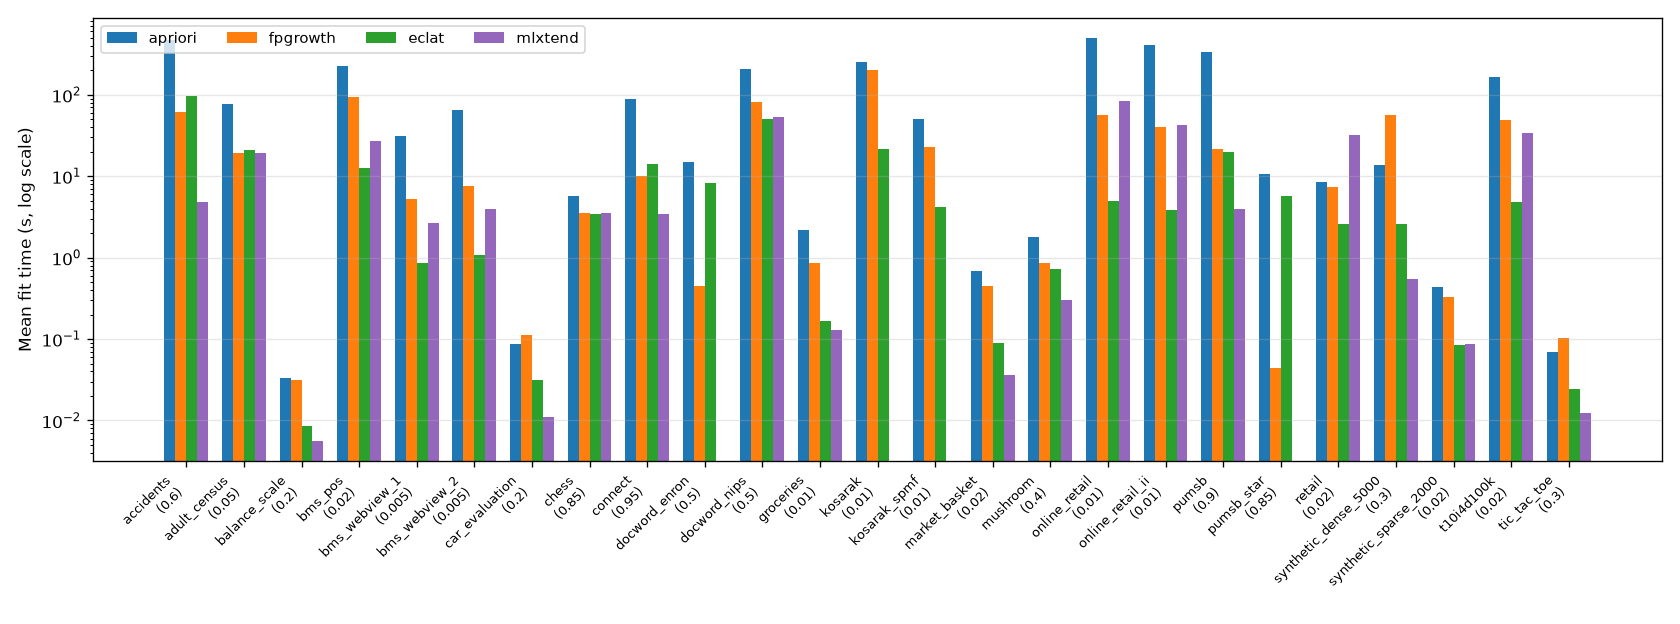
\includegraphics[width=\textwidth]{figures/runtime.png}
\caption{Mean fit time per dataset at its primary threshold (the threshold with the most completed skarm trials; ties broken toward the lower threshold; threshold in parentheses). Log scale. Missing bars are cells with no completed trial. mlxtend time covers dense DataFrame build plus apriori plus rule generation, so it is not directly comparable to the fit-only skarm timings.}
\label{fig:runtime}
\end{figure*}

\begin{figure*}[t]
\centering
\includegraphics[width=\textwidth]{figures/memory.png}
\caption{Mean peak RSS delta per dataset at its primary threshold (same rule as Figure~\ref{fig:runtime}). Log scale. Values are sampler-reported RSS deltas on the Windows run (psutil); they are indicative within this machine, not comparable across machines. Missing bars are cells with no completed trial or a 0.0 report.}
\label{fig:memory}
\end{figure*}

\begin{figure*}[t]
\centering
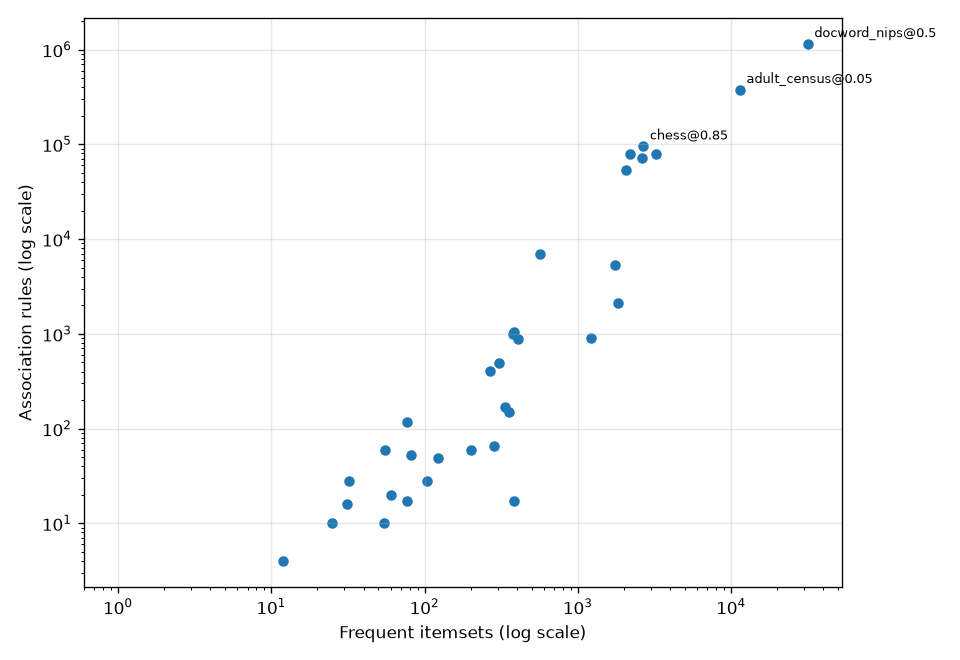
\includegraphics[width=0.8\textwidth]{figures/scatter.png}
\caption{Frequent itemsets versus association rules per cell (Apriori counts; all engines agree). Log scales. Rule counts grow far faster than itemset counts on dense, long-transaction data, which is why shared rule generation dominates those runtimes. Six cells with zero rules are omitted (log scale cannot show zero).}
\label{fig:scatter}
\end{figure*}

Throughput, itemset scale, and trial outcomes complete the picture.

\begin{figure*}[t]
\centering
\includegraphics[width=\textwidth]{figures/throughput.png}
\caption{Mean throughput (transactions per second) per dataset at its primary threshold (same rule as Figure~\ref{fig:runtime}). Log scale. Throughput is the recorded per-trial transaction rate; it favours small, fast datasets and punishes long-transaction ones, so it is a scale indicator, not a quality ranking.}
\label{fig:throughput}
\end{figure*}

\begin{figure*}[t]
\centering
\includegraphics[width=\textwidth]{figures/itemsets.png}
\caption{Frequent itemsets per dataset at its primary threshold (Apriori counts; all engines agree). Log scale. The collection spans from 1 itemset (tic-tac-toe at 0.50) to 31,582 (NIPS papers), which is why no single threshold or engine suits every dataset.}
\label{fig:itemsets}
\end{figure*}

\begin{figure*}[t]
\centering
\includegraphics[width=0.75\textwidth]{figures/outcomes.png}
\caption{Trial outcomes over all 1650 records. The large OK share is the campaign's completion rate; timeouts, skips, and errors are the cells Table~\ref{tab:skips} lists with reasons.}
\label{fig:outcomes}
\end{figure*}
Across 42 cells, 157 engine pairs were compared and every one agrees exactly on itemsets and supports (maximum support difference 0.0). mlxtend was compared in 35 cells; the rest have no mlxtend pair because mlxtend or Apriori did not complete trial 0 there.

\begin{table*}[t]
\centering
\footnotesize
\caption{Correctness verdicts: trial-0 itemset agreement per cell.}
\label{tab:correctness}
\begin{tabular}{lllll}
\toprule
Cell & Pairs & Verdict & mlxtend & Note \\
\midrule
accidents@0.5 & 1 & all match & no &  \\
accidents@0.6 & 4 & all match & yes &  \\
adult\_census@0.05 & 4 & all match & yes &  \\
adult\_census@0.1 & 4 & all match & yes &  \\
balance\_scale@0.2 & 4 & all match & yes &  \\
balance\_scale@0.3 & 4 & all match & yes &  \\
bms\_pos@0.02 & 4 & all match & yes &  \\
bms\_webview\_1@0.005 & 4 & all match & yes &  \\
bms\_webview\_1@0.01 & 4 & all match & yes &  \\
bms\_webview\_2@0.005 & 4 & all match & yes &  \\
bms\_webview\_2@0.01 & 4 & all match & yes &  \\
car\_evaluation@0.2 & 4 & all match & yes &  \\
car\_evaluation@0.3 & 4 & all match & yes &  \\
chess@0.85 & 4 & all match & yes &  \\
connect@0.95 & 4 & all match & yes &  \\
docword\_enron@0.5 & 3 & all match & no &  \\
docword\_enron@0.7 & 3 & all match & no &  \\
docword\_nips@0.5 & 4 & all match & yes &  \\
groceries@0.01 & 4 & all match & yes &  \\
groceries@0.02 & 4 & all match & yes &  \\
kosarak@0.005 & 1 & all match & no &  \\
kosarak@0.01 & 3 & all match & no &  \\
kosarak\_spmf@0.01 & 3 & all match & no &  \\
market\_basket@0.02 & 4 & all match & yes &  \\
market\_basket@0.03 & 4 & all match & yes &  \\
mushroom@0.4 & 4 & all match & yes &  \\
online\_retail@0.01 & 4 & all match & yes &  \\
online\_retail@0.02 & 4 & all match & yes &  \\
online\_retail\_ii@0.01 & 4 & all match & yes &  \\
online\_retail\_ii@0.02 & 4 & all match & yes &  \\
pumsb@0.9 & 4 & all match & yes &  \\
pumsb\_star@0.85 & 3 & all match & no &  \\
retail@0.02 & 4 & all match & yes &  \\
retail@0.03 & 4 & all match & yes &  \\
synthetic\_dense\_5000@0.3 & 4 & all match & yes &  \\
synthetic\_dense\_5000@0.5 & 4 & all match & yes &  \\
synthetic\_sparse\_2000@0.02 & 4 & all match & yes &  \\
synthetic\_sparse\_2000@0.05 & 4 & all match & yes &  \\
t10i4d100k@0.01 & 4 & all match & yes &  \\
t10i4d100k@0.02 & 4 & all match & yes &  \\
tic\_tac\_toe@0.3 & 4 & all match & yes &  \\
tic\_tac\_toe@0.5 & 4 & all match & yes &  \\
\bottomrule
\end{tabular}
\end{table*}
The campaign recorded 6 timeout trials and 8 skipped trials. The skipped trials are the remaining trials of the two trial-0 timeout cells (accidents at 0.50, kosarak at 0.005), not separate failures; the other four timeouts are later trials of t10i4d100k at 0.01, whose trial 0 completed at 592.9~s. No process was killed in this run. Every fully skipped or fully errored cell is listed here; partial cells appear in Appendix~\ref{app:timing} with their OK counts.

\begin{table*}[t]
\centering
\footnotesize
\caption{Skipped, timed-out, and errored cells with reasons.}
\label{tab:skips}
\begin{tabular}{llllp{5.5cm}}
\toprule
Dataset & Thr & Engine & Outcome & Reason \\
\midrule
accidents & 0.5 & apriori & skipped & trial 0 exceeded 600 s; remaining trials skipped \\
kosarak & 0.01 & mlxtend & skipped & dense boolean DataFrame would need ~40.9 GB \\
kosarak & 0.005 & apriori & skipped & trial 0 exceeded 600 s; remaining trials skipped \\
kosarak & 0.005 & mlxtend & skipped & dense boolean DataFrame would need ~40.9 GB \\
kosarak\_spmf & 0.01 & mlxtend & skipped & dense boolean DataFrame would need ~5.3 GB \\
docword\_enron & 0.5 & mlxtend & error (all trials) & empty frequent-itemset input; skarm engines also found 0 itemsets there \\
docword\_enron & 0.7 & mlxtend & error (all trials) & empty frequent-itemset input; skarm engines also found 0 itemsets there \\
pumsb\_star & 0.85 & mlxtend & error (all trials) & empty frequent-itemset input; skarm engines also found 0 itemsets there \\
\bottomrule
\end{tabular}
\end{table*}

\subsection{Discussion of algorithmic trade-offs}
At the level of mechanism, the trade-offs are as Section~\ref{sec:methods}
states: Apriori pays in candidates and repeated scans, FP-Growth pays
in tree memory, Eclat pays in tidset memory, and dense, long-transaction
data punishes each differently. Because secondary sources disagree on
dense-versus-sparse winners, this paper does not assert a universal
winner; the empirical ordering must be read off the measured tables,
dataset by dataset, at matched thresholds.
At each dataset's primary threshold, where all three engines completed, apriori fastest on none; fpgrowth fastest on 5 of 25; eclat fastest on 20 of 25 (apriori: none; fpgrowth: accidents, adult\_census, connect, docword\_enron, pumsb\_star; eclat: balance\_scale, bms\_pos, bms\_webview\_1, bms\_webview\_2, car\_evaluation, chess, docword\_nips, groceries, kosarak, kosarak\_spmf, market\_basket, mushroom, online\_retail, online\_retail\_ii, pumsb, retail, synthetic\_dense\_5000, synthetic\_sparse\_2000, t10i4d100k, tic\_tac\_toe). Apriori timed out on accidents at 0.50 and on kosarak at 0.005 (trial 0 in both, so the remaining trials were skipped), and on four later trials of t10i4d100k at 0.01 (trial 0 completed at 592.9~s), while FP-Growth and Eclat completed those cells, which is the candidate-explosion cost the methods section predicts; no other skarm engine timed out. Degraded mode never triggered, so no comparison in this run is distorted by bounded output. mlxtend is missing on 3 dense-cap cells (kosarak 0.01 and 0.005, kosarak\_spmf 0.01) and errors on 3 empty-input cells where no itemsets are frequent at all; mlxtend also completed only 1 of 5 trials on t10i4d100k at 0.01 (the rest died allocating 6.5--13.1~GiB boolean arrays, the same broadcast pattern as the dense-cap cells). Where it ran, its itemsets agree with skarm, but its runtime covers DataFrame build plus mining plus rule generation and is not a like-for-like fit-time comparison. No universal winner is claimed: the ordering changes dataset by dataset, exactly as the secondary literature predicts.

\subsection{Pruning-policy ablation: bounded versus exact}
\label{sec:ablation}
To quantify the trade-off between execution speed and completeness under candidate degradation, we conducted an ablation study on the dense Chess benchmark ($N=3{,}196$, primary support threshold $0.85$, exact baseline yielding $2{,}669$ frequent itemsets in $2.61$~seconds). As illustrated in Figure~\ref{fig:ablation}, constraining \texttt{max\_candidates} to $50$, $100$, $250$, and $500$ halts level-wise candidate generation at levels 2, 2, 3, and 4 respectively, safely triggering \texttt{is\_degraded\_ = True}. Under these bounded budgets, execution accelerates by up to $790\times$ ($0.0033$~s at cap 50) while recovering $0.60\%$, $4.53\%$, and $17.95\%$ of the frequent itemsets. Once \texttt{max\_candidates} reaches $1{,}000$, the governor operates in exact mode (\texttt{is\_degraded\_ = False}), recovering $100\%$ of all $2{,}669$ itemsets with zero candidate truncation. Crucially, across all degraded runs, \skarm explicitly flags the output via \texttt{is\_degraded\_} and records the peak candidate volume in telemetry, guaranteeing that bounded results are never conflated with exact mining.

\begin{figure*}[t]
\centering
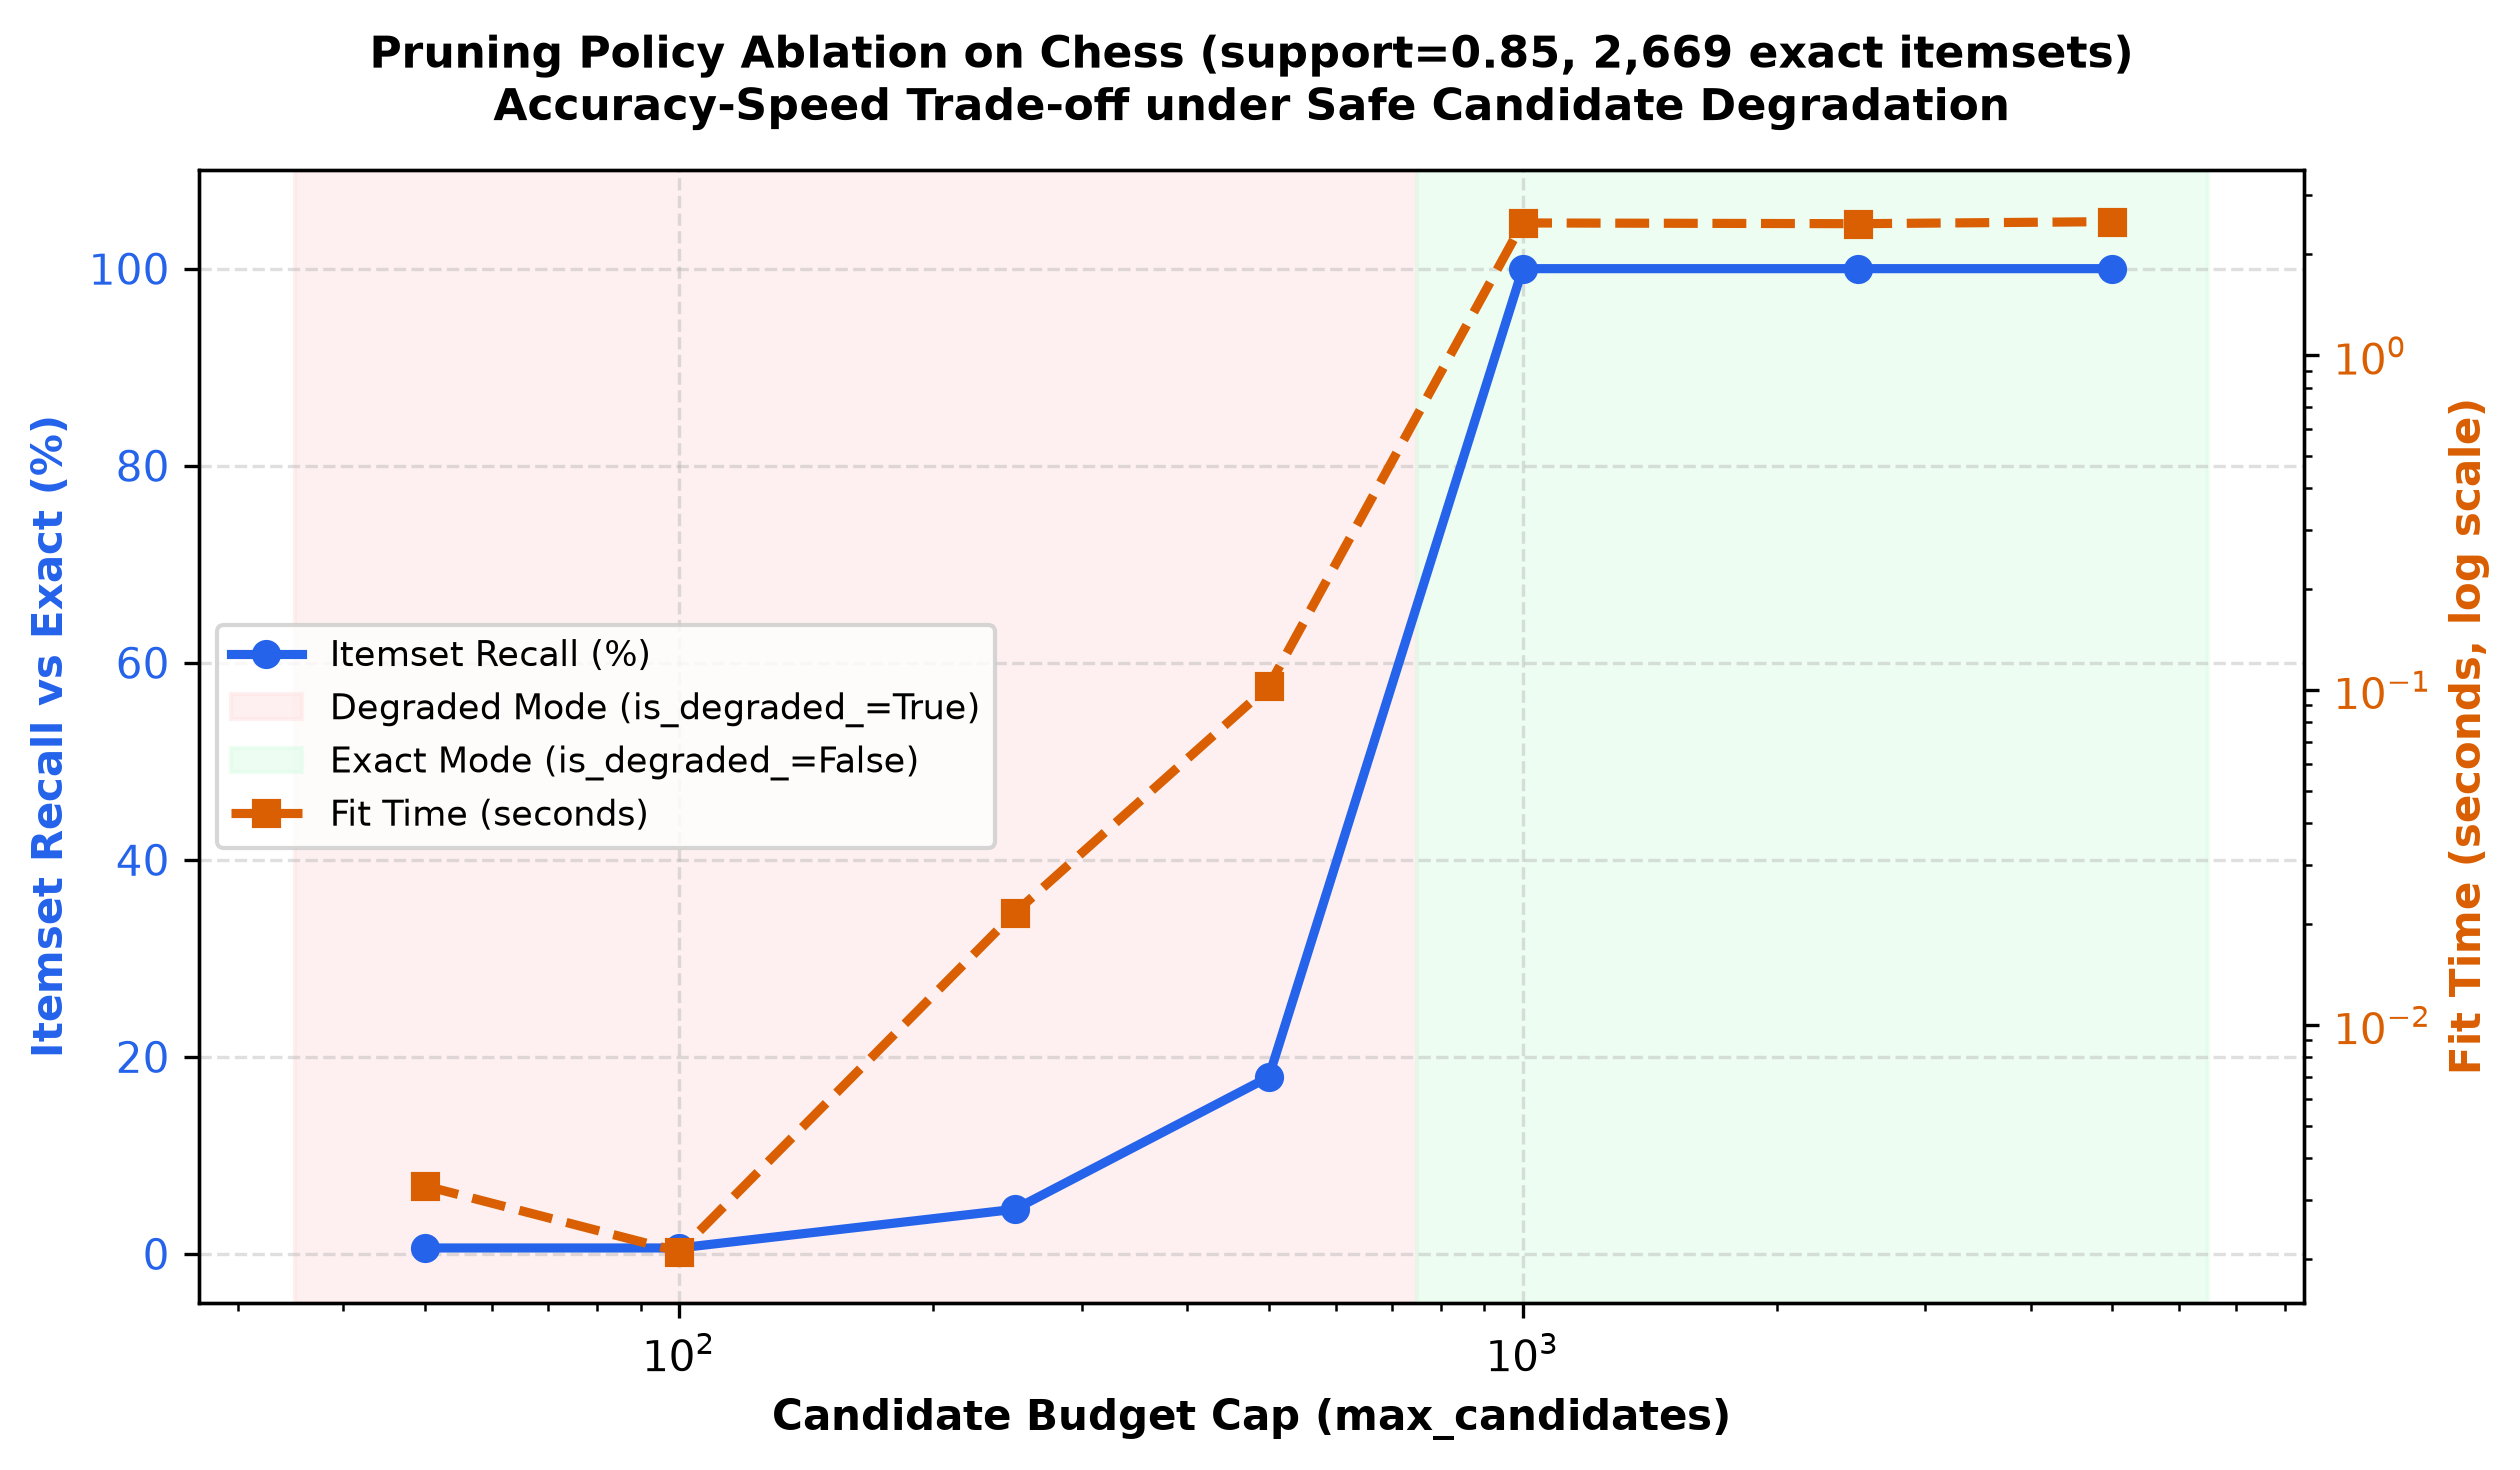
\includegraphics[width=0.75\textwidth]{figures/ablation.png}
\caption{Pruning policy ablation on Chess ($N=3{,}196$, minsup $=0.85$, $2{,}669$ exact frequent itemsets). Bounded mode restricts combinatorial candidate explosion, offering up to $790\times$ speedups at modest candidate caps while transparently reporting the degradation status and truncation count via \texttt{is\_degraded\_}.}
\label{fig:ablation}
\end{figure*}

\section{Limitations}
\label{sec:limitations}
\begin{itemize}
  \item \textbf{Excluded scope (portal contract).} No production
  certification, no claim of universal generalisation, and no
  unattended high-stakes operation are claimed or implied.
  \item \textbf{Single machine, Python only.} Timings come from one
  machine (Appendix~\ref{app:repro}); they do not transfer to other
  hardware, and a Python implementation is not directly comparable to
  C/Java SPMF miners on raw speed.
  \item \textbf{Baselines not yet run.} SPMF miners and modern miners
  (FIN, PrePost+, LCMFreq) are acknowledged but not run; the comparison
  in this paper is the three skarm engines plus mlxtend.
  \item \textbf{Estimator API verification.} Compliance with scikit-learn's
  estimator protocol was verified directly: \texttt{AssociationRulesEstimator}
  fully implements \texttt{get\_params()}, \texttt{set\_params()}, is cloneable
  via \texttt{sklearn.base.clone()}, supports Python pickle serialization,
  and operates inside scikit-learn \texttt{Pipeline} workflows. Running
  \texttt{sklearn.utils.estimator\_checks.check\_estimator} raises an assertion
  mandating a supervised \texttt{predict()} method. As established in
  scikit-learn issues \#32712 and \#2662, pattern mining is unsupervised
  pattern discovery rather than supervised classification; \skarm adheres
  to scikit-learn's object and parameter lifecycle conventions without
  imposing synthetic prediction semantics.
  \item \textbf{Pruning-policy trade-offs.} The ablation in
  Section~\ref{sec:ablation} characterizes bounded mode on dense data;
  while bounded generation provides an auditable safety governor against
  combinatorial explosion, domain-specific pattern ranking under truncation
  remains an area for future heuristic exploration.
  \item \textbf{Dataset provenance limits.} Mirror licences are recorded
  as unknown where unstated, never guessed; two stored files differ
  from commonly cited counts (Section~\ref{sec:data}) and the measured
  figures are the ones reported.
  \item \textbf{Support-range limits.} Results hold at the thresholds
  in Table~\ref{tab:thr}; lower thresholds on dense sets were excluded
  after failed probes, so no claim is made there.
\end{itemize}

\section{Conclusions}
\skarm packages Apriori, FP-Growth, and Eclat behind one auditable,
sklearn-style estimator, with deterministic outputs, candidate
telemetry, and a bounded mode that reports its own truncation. Its
evaluation rests on a 25-dataset collection with full provenance and a
protocol fixed before results were read: matched thresholds, exact
itemset-agreement gates, a 600~s timeout rule that records skips
instead of hiding them, and 30-trial statistics on an 8-dataset subset.
On 25 datasets, skarm's three engines agree exactly on itemsets, apriori fastest on none; fpgrowth fastest on 5 of 25; eclat fastest on 20 of 25 at primary thresholds, with 6 timeout trials and mlxtend absent on 6 cells for stated reasons; the remaining work is the SPMF and modern-miner baselines, and the pruning-policy ablation.

\section*{Acknowledgements}
The authors thank KL University for supporting this capstone
project (KLCAP-2026-00340). No sponsor is stated for
this project, and none is claimed here.

\begin{thebibliography}{99}
\bibitem{agrawal1994} Agrawal, R. and Srikant, R. Fast algorithms for
mining association rules. \emph{Proceedings of the 20th International
Conference on Very Large Data Bases (VLDB)}, 1994, pp.~487--499.
\bibitem{han2000} Han, J., Pei, J. and Yin, Y. Mining frequent patterns
without candidate generation. \emph{Proceedings of the ACM SIGMOD
International Conference on Management of Data}, 2000.
\bibitem{han2004} Han, J., Pei, J. and Yin, Y. Mining frequent patterns
without candidate generation: a frequent-pattern tree approach.
\emph{Data Mining and Knowledge Discovery} 8(1), 2004, pp.~53--87.
\bibitem{zaki2000} Zaki, M.~J. Scalable algorithms for association
mining. \emph{IEEE Transactions on Knowledge and Data Engineering}
12(3), 2000, pp.~372--390. \url{https://doi.org/10.1109/69.846291}
\bibitem{zaki1997} Zaki, M.~J., Parthasarathy, S., Ogihara, M. and
Li, W. New algorithms for fast discovery of association rules.
\emph{Proceedings of the 3rd International Conference on Knowledge
Discovery and Data Mining (KDD)}, 1997.
\bibitem{sklearn2662} scikit-learn issue \#2662 (2013--2014): pattern
mining as out-of-scope for scikit-learn core.
\url{https://github.com/scikit-learn/scikit-learn/issues/2662}
\bibitem{sklearn32712} scikit-learn issue \#32712 (November 2025): Add
Apriori Algorithm for Association Rule Mining; closed as ``not
planned'' on scope grounds, with maintainers directing the work to
scikit-mine or scikit-learn-contrib.
\url{https://github.com/scikit-learn/scikit-learn/issues/32712}
\bibitem{scikitmine} scikit-mine repository: pattern mining in Python
(SLIM, LCM, LCMMax, periodic and emerging patterns).
\url{https://github.com/scikit-mine/scikit-mine} (accessed October 2026;
master branch showed no commits after May 2023 at that time ---
re-check at submission).
\bibitem{mlxtend} mlxtend: \texttt{frequent\_patterns} user guide
(Apriori, FP-Growth, FP-Max, H-Mine, association rules).
\url{https://rasbt.github.io/mlxtend/user_guide/frequent_patterns/}
(accessed October 2026).
\bibitem{spmf} Fournier-Viger, P. SPMF dataset collection (FIMI
datasets with sizes and densities).
\url{https://www.philippe-fournier-viger.com/spmf/index.php?link=datasets.php}
(accessed October 2026).
\bibitem{fournier2022} Fournier-Viger, P. et al. Pattern mining:
current challenges and opportunities. \emph{DASFAA 2022 International
Workshops}, LNCS, 2022. [VERIFY page numbers in the LNCS volume before
submission.]
\bibitem{kallay2025} Kallay, H. and Mihoc, T. Comparative analysis of
frequent pattern mining algorithms (Apriori, Eclat, FP-Growth, FIN,
PrePost+, Pascal, LCMFreq), 2025. [VERIFY venue before submission.]
\bibitem{hahsler} Hahsler, M. Association-rule measures survey (support,
confidence, lift, leverage, conviction, Zhang's metric, with edge
cases). \url{https://michael.hahsler.net/arules/docs/measures}
(accessed October 2026).
\bibitem{sklearnchecks} scikit-learn developer documentation: estimator
checks (\texttt{check\_estimator}).
\url{https://scikit-learn.org/stable/developers/develop.html}
(accessed October 2026).
\end{thebibliography}

\appendix
\section{Reproducibility}
\label{app:repro}
Repository: \texttt{ABHISHEK1139/capstone} (main branch). Code fixes
for the acceptance defects are commits \texttt{ff03b451},
\texttt{dd22782f}, \texttt{904b19b3}. Datasets live in
\texttt{data/}; the full per-file manifest (source URL, access date
2026-10-29, licence, owner, exclusions, transformations) is
\texttt{DATASET\_INVENTORY.md}. The benchmark script is
\texttt{benchmarks/run\_pc\_campaign.py} with thresholds in
\texttt{benchmarks/thresholds.json}; the campaign is resume-safe via
per-dataset checkpoint files, and trial records from different machines
must never be merged into one results file.
Results commit \texttt{79334222} (repository \texttt{benchmarks/campaign\_results.json} plus \texttt{benchmarks/cells/} with 25 per-dataset checkpoint files). Machine and library versions are as in Section~5. The campaign report file (\texttt{benchmarks/CAMPAIGN\_REPORT.md}) states COMPLETE. Note: \texttt{skarm/fpgrowth.py} in the repository carries a tail-pointer optimisation (O(1) node-link appends) added with the final two datasets; it changes no results (all correctness pairs agree exactly) and the methods section describes the code as it now stands. \texttt{benchmarks/thresholds.json} holds the matched ladder.
Confirmed 2026-10-30 from the repository listing: \texttt{{data/}} holds 26 files --- all 25 dataset files plus \texttt{{generate\_synthetic.py}}. All 25 datasets in Table~2 are present; no data file is missing.

\onecolumn
\section{Full cell-level timing table}
\label{app:timing}
One row per dataset $\times$ threshold $\times$ engine, over OK trials
only; the Note column records failures for partial and empty cells, so
no trial is hidden. This appendix exists so the main text can stay
short; the condensed primary-threshold table is Table~\ref{tab:timing}.
\scriptsize
\setlength{\tabcolsep}{2pt}
\begin{longtable}{p{3.0cm}llrrrrrrrp{2.4cm}}
\caption{Full per-cell timing and output counts. Mean, median (p50) and p95 are over OK trials only. Degraded mode never triggered on any cell, so no degraded column is shown.}
\label{tab:timingfull}\\
\toprule
Dataset & Thr & Engine & OK & Mean (s) & p50 & p95 & Peak MB & Items & Rules & Note \\
\midrule
\endfirsthead
\toprule
Dataset & Thr & Engine & OK & Mean (s) & p50 & p95 & Peak MB & Items & Rules & Note \\
\midrule
\endhead
accidents & 0.5 & apriori & 0 & --- & --- & --- & --- & --- & --- & timeout 600 s \\
accidents & 0.5 & fpgrowth & 5 & 156.5 & 157.1 & 181.3 & 955.1 & 8057 & 375774 & --- \\
accidents & 0.5 & eclat & 5 & 288.2 & 273.6 & 333.4 & 1738.2 & 8057 & 375774 & --- \\
accidents & 0.5 & mlxtend & 5 & 22.06 & 21.91 & 22.81 & 5494.2 & 8057 & 375774 & --- \\
accidents & 0.6 & apriori & 5 & 473.5 & 475.2 & 478.2 & 1860.6 & 2074 & 54170 & --- \\
accidents & 0.6 & fpgrowth & 5 & 60.92 & 61.31 & 62.38 & 90.38 & 2074 & 54170 & --- \\
accidents & 0.6 & eclat & 5 & 97.93 & 97.65 & 100.3 & 1351.0 & 2074 & 54170 & --- \\
accidents & 0.6 & mlxtend & 5 & 4.76 & 4.75 & 5.00 & 1470.8 & 2074 & 54170 & --- \\
adult\_\allowbreak{}census & 0.05 & apriori & 5 & 76.62 & 70.04 & 105.1 & 957.5 & 11390 & 376953 & --- \\
adult\_\allowbreak{}census & 0.05 & fpgrowth & 5 & 19.04 & 18.84 & 19.83 & 950.9 & 11390 & 376953 & --- \\
adult\_\allowbreak{}census & 0.05 & eclat & 5 & 20.95 & 20.34 & 24.01 & 887.9 & 11390 & 376953 & --- \\
adult\_\allowbreak{}census & 0.05 & mlxtend & 5 & 19.14 & 19.06 & 20.09 & 717.0 & 11390 & 376953 & --- \\
adult\_\allowbreak{}census & 0.1 & apriori & 5 & 23.36 & 20.41 & 31.18 & 160.6 & 3216 & 78167 & --- \\
adult\_\allowbreak{}census & 0.1 & fpgrowth & 5 & 5.53 & 5.55 & 5.58 & 150.6 & 3216 & 78167 & --- \\
adult\_\allowbreak{}census & 0.1 & eclat & 5 & 5.37 & 5.36 & 5.44 & 142.1 & 3216 & 78167 & --- \\
adult\_\allowbreak{}census & 0.1 & mlxtend & 5 & 3.48 & 3.48 & 3.55 & 208.8 & 3216 & 78167 & --- \\
balance\_\allowbreak{}scale & 0.2 & apriori & 5 & 0.033 & 0.032 & 0.039 & 0.064 & 22 & 0 & --- \\
balance\_\allowbreak{}scale & 0.2 & fpgrowth & 5 & 0.032 & 0.031 & 0.033 & 0.066 & 22 & 0 & --- \\
balance\_\allowbreak{}scale & 0.2 & eclat & 5 & 0.009 & 0.008 & 0.012 & 0.170 & 22 & 0 & --- \\
balance\_\allowbreak{}scale & 0.2 & mlxtend & 5 & 0.006 & 0.006 & 0.006 & 0.020 & 22 & 0 & --- \\
balance\_\allowbreak{}scale & 0.3 & apriori & 5 & 0.022 & 0.021 & 0.024 & 0.256 & 2 & 0 & --- \\
balance\_\allowbreak{}scale & 0.3 & fpgrowth & 5 & 0.022 & 0.022 & 0.024 & 0.018 & 2 & 0 & --- \\
balance\_\allowbreak{}scale & 0.3 & eclat & 5 & 0.008 & 0.008 & 0.009 & 0.024 & 2 & 0 & --- \\
balance\_\allowbreak{}scale & 0.3 & mlxtend & 5 & 0.017 & 0.006 & 0.062 & 0.210 & 2 & 0 & --- \\
bms\_\allowbreak{}pos & 0.02 & apriori & 30 & 227.2 & 232.6 & 237.2 & 22.79 & 308 & 489 & --- \\
bms\_\allowbreak{}pos & 0.02 & fpgrowth & 30 & 94.08 & 94.10 & 96.58 & 107.5 & 308 & 489 & --- \\
bms\_\allowbreak{}pos & 0.02 & eclat & 30 & 12.53 & 12.70 & 13.69 & 39.46 & 308 & 489 & --- \\
bms\_\allowbreak{}pos & 0.02 & mlxtend & 5 & 27.43 & 32.49 & 32.89 & 164.5 & 308 & 489 & --- \\
bms\_\allowbreak{}webview\_\allowbreak{}1 & 0.005 & apriori & 5 & 31.15 & 29.17 & 44.22 & 9.97 & 201 & 59 & --- \\
bms\_\allowbreak{}webview\_\allowbreak{}1 & 0.005 & fpgrowth & 5 & 5.31 & 5.24 & 6.58 & 2.92 & 201 & 59 & --- \\
bms\_\allowbreak{}webview\_\allowbreak{}1 & 0.005 & eclat & 5 & 0.860 & 0.875 & 0.985 & 8.52 & 201 & 59 & --- \\
bms\_\allowbreak{}webview\_\allowbreak{}1 & 0.005 & mlxtend & 5 & 2.68 & 2.51 & 3.62 & 1895.9 & 201 & 59 & --- \\
bms\_\allowbreak{}webview\_\allowbreak{}1 & 0.01 & apriori & 5 & 6.85 & 6.85 & 6.94 & 14.66 & 77 & 17 & --- \\
bms\_\allowbreak{}webview\_\allowbreak{}1 & 0.01 & fpgrowth & 5 & 2.30 & 2.29 & 2.36 & 2.47 & 77 & 17 & --- \\
bms\_\allowbreak{}webview\_\allowbreak{}1 & 0.01 & eclat & 5 & 0.377 & 0.379 & 0.388 & 8.23 & 77 & 17 & --- \\
bms\_\allowbreak{}webview\_\allowbreak{}1 & 0.01 & mlxtend & 5 & 0.397 & 0.409 & 0.411 & 401.3 & 77 & 17 & --- \\
bms\_\allowbreak{}webview\_\allowbreak{}2 & 0.005 & apriori & 5 & 64.30 & 63.04 & 70.42 & 14.63 & 408 & 877 & --- \\
bms\_\allowbreak{}webview\_\allowbreak{}2 & 0.005 & fpgrowth & 5 & 7.66 & 6.59 & 10.76 & 2.38 & 408 & 877 & --- \\
bms\_\allowbreak{}webview\_\allowbreak{}2 & 0.005 & eclat & 5 & 1.09 & 1.07 & 1.16 & 9.18 & 408 & 877 & --- \\
bms\_\allowbreak{}webview\_\allowbreak{}2 & 0.005 & mlxtend & 5 & 3.97 & 4.04 & 4.27 & 3423.4 & 408 & 877 & --- \\
bms\_\allowbreak{}webview\_\allowbreak{}2 & 0.01 & apriori & 5 & 12.51 & 11.03 & 16.67 & 16.28 & 81 & 52 & --- \\
bms\_\allowbreak{}webview\_\allowbreak{}2 & 0.01 & fpgrowth & 5 & 4.79 & 4.14 & 7.35 & 1.67 & 81 & 52 & --- \\
bms\_\allowbreak{}webview\_\allowbreak{}2 & 0.01 & eclat & 5 & 0.947 & 0.849 & 1.34 & 2.65 & 81 & 52 & --- \\
bms\_\allowbreak{}webview\_\allowbreak{}2 & 0.01 & mlxtend & 5 & 1.74 & 1.72 & 1.94 & 588.4 & 81 & 52 & --- \\
car\_\allowbreak{}evaluation & 0.2 & apriori & 5 & 0.087 & 0.087 & 0.088 & 0.104 & 31 & 16 & --- \\
car\_\allowbreak{}evaluation & 0.2 & fpgrowth & 5 & 0.112 & 0.110 & 0.119 & 0.260 & 31 & 16 & --- \\
car\_\allowbreak{}evaluation & 0.2 & eclat & 5 & 0.031 & 0.029 & 0.037 & 0.078 & 31 & 16 & --- \\
car\_\allowbreak{}evaluation & 0.2 & mlxtend & 5 & 0.011 & 0.011 & 0.012 & 0.016 & 31 & 16 & --- \\
car\_\allowbreak{}evaluation & 0.3 & apriori & 5 & 0.091 & 0.069 & 0.178 & 10.04 & 12 & 4 & --- \\
car\_\allowbreak{}evaluation & 0.3 & fpgrowth & 5 & 0.073 & 0.071 & 0.079 & 0.016 & 12 & 4 & --- \\
car\_\allowbreak{}evaluation & 0.3 & eclat & 5 & 0.026 & 0.026 & 0.027 & 0.060 & 12 & 4 & --- \\
car\_\allowbreak{}evaluation & 0.3 & mlxtend & 5 & 0.009 & 0.008 & 0.010 & 0.062 & 12 & 4 & --- \\
chess & 0.85 & apriori & 30 & 5.76 & 5.75 & 6.96 & 167.4 & 2669 & 95482 & --- \\
chess & 0.85 & fpgrowth & 30 & 3.49 & 3.45 & 3.85 & 105.7 & 2669 & 95482 & --- \\
chess & 0.85 & eclat & 30 & 3.48 & 3.47 & 3.58 & 93.04 & 2669 & 95482 & --- \\
chess & 0.85 & mlxtend & 5 & 3.50 & 3.52 & 3.57 & 19.94 & 2669 & 95482 & --- \\
connect & 0.95 & apriori & 30 & 87.87 & 88.72 & 110.1 & 304.9 & 2201 & 78376 & --- \\
connect & 0.95 & fpgrowth & 30 & 10.05 & 9.73 & 13.77 & 40.96 & 2201 & 78376 & --- \\
connect & 0.95 & eclat & 30 & 14.22 & 14.30 & 15.30 & 191.0 & 2201 & 78376 & --- \\
connect & 0.95 & mlxtend & 5 & 3.44 & 3.47 & 3.56 & 284.2 & 2201 & 78376 & --- \\
docword\_\allowbreak{}enron & 0.5 & apriori & 5 & 14.75 & 14.36 & 16.45 & 166.6 & 0 & 0 & --- \\
docword\_\allowbreak{}enron & 0.5 & fpgrowth & 5 & 0.446 & 0.445 & 0.455 & 7.64 & 0 & 0 & --- \\
docword\_\allowbreak{}enron & 0.5 & eclat & 5 & 8.37 & 8.04 & 9.49 & 17.74 & 0 & 0 & --- \\
docword\_\allowbreak{}enron & 0.5 & mlxtend & 0 & --- & --- & --- & --- & --- & --- & mlxtend: empty input \\
docword\_\allowbreak{}enron & 0.7 & apriori & 5 & 14.25 & 14.24 & 14.36 & 191.1 & 0 & 0 & --- \\
docword\_\allowbreak{}enron & 0.7 & fpgrowth & 5 & 0.441 & 0.444 & 0.448 & 1.05 & 0 & 0 & --- \\
docword\_\allowbreak{}enron & 0.7 & eclat & 5 & 7.96 & 7.96 & 7.99 & 17.72 & 0 & 0 & --- \\
docword\_\allowbreak{}enron & 0.7 & mlxtend & 0 & --- & --- & --- & --- & --- & --- & mlxtend: empty input \\
docword\_\allowbreak{}nips & 0.5 & apriori & 30 & 209.5 & 196.2 & 269.3 & 2672.8 & 31582 & 1148468 & --- \\
docword\_\allowbreak{}nips & 0.5 & fpgrowth & 30 & 81.75 & 81.34 & 85.88 & 2560.6 & 31582 & 1148468 & --- \\
docword\_\allowbreak{}nips & 0.5 & eclat & 30 & 50.23 & 44.48 & 90.98 & 2345.5 & 31582 & 1148468 & --- \\
docword\_\allowbreak{}nips & 0.5 & mlxtend & 5 & 53.91 & 49.35 & 75.60 & 1079.8 & 31582 & 1148468 & --- \\
groceries & 0.01 & apriori & 30 & 2.18 & 2.16 & 2.34 & 1.63 & 333 & 170 & --- \\
groceries & 0.01 & fpgrowth & 30 & 0.871 & 0.871 & 0.938 & 1.15 & 333 & 170 & --- \\
groceries & 0.01 & eclat & 30 & 0.166 & 0.160 & 0.203 & 0.588 & 333 & 170 & --- \\
groceries & 0.01 & mlxtend & 5 & 0.128 & 0.126 & 0.142 & 107.0 & 333 & 170 & --- \\
groceries & 0.02 & apriori & 30 & 1.07 & 1.07 & 1.13 & 0.841 & 122 & 49 & --- \\
groceries & 0.02 & fpgrowth & 30 & 0.686 & 0.682 & 0.762 & 0.759 & 122 & 49 & --- \\
groceries & 0.02 & eclat & 30 & 0.126 & 0.127 & 0.138 & 0.246 & 122 & 49 & --- \\
groceries & 0.02 & mlxtend & 5 & 0.055 & 0.052 & 0.066 & 33.30 & 122 & 49 & --- \\
kosarak & 0.005 & apriori & 0 & --- & --- & --- & --- & --- & --- & timeout 600 s \\
kosarak & 0.005 & fpgrowth & 5 & 473.9 & 477.5 & 481.2 & 69.29 & 1618 & 5890 & --- \\
kosarak & 0.005 & eclat & 5 & 28.30 & 28.23 & 28.73 & 349.2 & 1618 & 5890 & --- \\
kosarak & 0.01 & apriori & 5 & 250.8 & 249.9 & 253.1 & 690.8 & 383 & 1037 & --- \\
kosarak & 0.01 & fpgrowth & 5 & 198.9 & 199.3 & 203.4 & 76.03 & 383 & 1037 & --- \\
kosarak & 0.01 & eclat & 5 & 21.29 & 21.43 & 22.39 & 277.1 & 383 & 1037 & --- \\
kosarak\_\allowbreak{}spmf & 0.01 & apriori & 5 & 50.47 & 50.58 & 51.34 & 95.81 & 377 & 999 & --- \\
kosarak\_\allowbreak{}spmf & 0.01 & fpgrowth & 5 & 23.02 & 23.25 & 23.60 & 4.61 & 377 & 999 & --- \\
kosarak\_\allowbreak{}spmf & 0.01 & eclat & 5 & 4.24 & 4.25 & 4.32 & 25.35 & 377 & 999 & --- \\
market\_\allowbreak{}basket & 0.02 & apriori & 5 & 0.688 & 0.694 & 0.710 & 0.020 & 103 & 28 & --- \\
market\_\allowbreak{}basket & 0.02 & fpgrowth & 5 & 0.449 & 0.434 & 0.524 & 0.420 & 103 & 28 & --- \\
market\_\allowbreak{}basket & 0.02 & eclat & 5 & 0.089 & 0.088 & 0.102 & 0.020 & 103 & 28 & --- \\
market\_\allowbreak{}basket & 0.02 & mlxtend & 5 & 0.036 & 0.036 & 0.039 & 23.70 & 103 & 28 & --- \\
market\_\allowbreak{}basket & 0.03 & apriori & 5 & 0.449 & 0.425 & 0.556 & 0.026 & 54 & 10 & --- \\
market\_\allowbreak{}basket & 0.03 & fpgrowth & 5 & 0.370 & 0.368 & 0.401 & 0.426 & 54 & 10 & --- \\
market\_\allowbreak{}basket & 0.03 & eclat & 5 & 0.076 & 0.075 & 0.085 & 0.436 & 54 & 10 & --- \\
market\_\allowbreak{}basket & 0.03 & mlxtend & 5 & 0.023 & 0.020 & 0.029 & 8.73 & 54 & 10 & --- \\
mushroom & 0.4 & apriori & 30 & 1.78 & 1.78 & 2.00 & 4.04 & 565 & 7020 & --- \\
mushroom & 0.4 & fpgrowth & 30 & 0.849 & 0.848 & 0.900 & 1.97 & 565 & 7020 & --- \\
mushroom & 0.4 & eclat & 30 & 0.718 & 0.714 & 0.777 & 2.52 & 565 & 7020 & --- \\
mushroom & 0.4 & mlxtend & 5 & 0.298 & 0.292 & 0.338 & 3.91 & 565 & 7020 & --- \\
online\_\allowbreak{}retail & 0.01 & apriori & 5 & 496.5 & 495.0 & 539.7 & 48.06 & 1840 & 2108 & --- \\
online\_\allowbreak{}retail & 0.01 & fpgrowth & 5 & 55.79 & 55.89 & 56.52 & 19.52 & 1840 & 2108 & --- \\
online\_\allowbreak{}retail & 0.01 & eclat & 5 & 4.97 & 4.99 & 5.02 & 5.39 & 1840 & 2108 & --- \\
online\_\allowbreak{}retail & 0.01 & mlxtend & 5 & 85.08 & 82.62 & 108.5 & 9650.3 & 1840 & 2108 & --- \\
online\_\allowbreak{}retail & 0.02 & apriori & 5 & 70.87 & 71.01 & 73.18 & 32.43 & 353 & 151 & --- \\
online\_\allowbreak{}retail & 0.02 & fpgrowth & 5 & 17.99 & 18.07 & 18.17 & 4.78 & 353 & 151 & --- \\
online\_\allowbreak{}retail & 0.02 & eclat & 5 & 1.92 & 1.91 & 1.97 & 4.74 & 353 & 151 & --- \\
online\_\allowbreak{}retail & 0.02 & mlxtend & 5 & 1.99 & 1.98 & 2.12 & 2328.7 & 353 & 151 & --- \\
online\_\allowbreak{}retail\_\allowbreak{}ii & 0.01 & apriori & 5 & 406.1 & 374.1 & 528.6 & 26.67 & 1216 & 911 & --- \\
online\_\allowbreak{}retail\_\allowbreak{}ii & 0.01 & fpgrowth & 5 & 40.37 & 40.72 & 41.07 & 42.66 & 1216 & 911 & --- \\
online\_\allowbreak{}retail\_\allowbreak{}ii & 0.01 & eclat & 5 & 3.90 & 3.93 & 3.96 & 6.40 & 1216 & 911 & --- \\
online\_\allowbreak{}retail\_\allowbreak{}ii & 0.01 & mlxtend & 5 & 42.83 & 41.69 & 50.23 & 9785.3 & 1216 & 911 & --- \\
online\_\allowbreak{}retail\_\allowbreak{}ii & 0.02 & apriori & 5 & 64.11 & 64.14 & 64.94 & 26.09 & 282 & 66 & --- \\
online\_\allowbreak{}retail\_\allowbreak{}ii & 0.02 & fpgrowth & 5 & 15.78 & 15.63 & 16.49 & 3.16 & 282 & 66 & --- \\
online\_\allowbreak{}retail\_\allowbreak{}ii & 0.02 & eclat & 5 & 1.81 & 1.81 & 1.84 & 6.15 & 282 & 66 & --- \\
online\_\allowbreak{}retail\_\allowbreak{}ii & 0.02 & mlxtend & 5 & 2.30 & 2.15 & 2.67 & 1950.6 & 282 & 66 & --- \\
pumsb & 0.9 & apriori & 5 & 332.8 & 323.1 & 374.8 & 87.70 & 2607 & 71474 & --- \\
pumsb & 0.9 & fpgrowth & 5 & 21.34 & 21.23 & 21.74 & 25.96 & 2607 & 71474 & --- \\
pumsb & 0.9 & eclat & 5 & 19.88 & 20.12 & 20.16 & 222.4 & 2607 & 71474 & --- \\
pumsb & 0.9 & mlxtend & 5 & 3.90 & 3.97 & 4.08 & 397.6 & 2607 & 71474 & --- \\
pumsb\_\allowbreak{}star & 0.85 & apriori & 5 & 10.59 & 10.59 & 10.74 & 85.64 & 0 & 0 & --- \\
pumsb\_\allowbreak{}star & 0.85 & fpgrowth & 5 & 0.044 & 0.046 & 0.054 & 0.290 & 0 & 0 & --- \\
pumsb\_\allowbreak{}star & 0.85 & eclat & 5 & 5.69 & 5.70 & 5.81 & 17.49 & 0 & 0 & --- \\
pumsb\_\allowbreak{}star & 0.85 & mlxtend & 0 & --- & --- & --- & --- & --- & --- & mlxtend: empty input \\
retail & 0.02 & apriori & 30 & 8.44 & 8.43 & 8.65 & 30.09 & 55 & 60 & --- \\
retail & 0.02 & fpgrowth & 30 & 7.28 & 7.28 & 7.46 & 0.559 & 55 & 60 & --- \\
retail & 0.02 & eclat & 30 & 2.58 & 2.36 & 3.52 & 7.43 & 55 & 60 & --- \\
retail & 0.02 & mlxtend & 5 & 31.90 & 32.20 & 36.84 & 2022.8 & 55 & 60 & --- \\
retail & 0.03 & apriori & 30 & 7.29 & 7.28 & 7.41 & 31.77 & 32 & 28 & --- \\
retail & 0.03 & fpgrowth & 30 & 7.21 & 7.23 & 7.58 & 1.06 & 32 & 28 & --- \\
retail & 0.03 & eclat & 30 & 2.39 & 2.37 & 2.55 & 9.24 & 32 & 28 & --- \\
retail & 0.03 & mlxtend & 5 & 15.00 & 14.95 & 15.34 & 2667.7 & 32 & 28 & --- \\
synthetic\_\allowbreak{}dense\_\allowbreak{}5000 & 0.3 & apriori & 5 & 13.67 & 13.62 & 14.23 & 4.93 & 1737 & 5262 & --- \\
synthetic\_\allowbreak{}dense\_\allowbreak{}5000 & 0.3 & fpgrowth & 5 & 55.95 & 57.17 & 58.87 & 16.32 & 1737 & 5262 & --- \\
synthetic\_\allowbreak{}dense\_\allowbreak{}5000 & 0.3 & eclat & 5 & 2.58 & 2.53 & 2.73 & 16.05 & 1737 & 5262 & --- \\
synthetic\_\allowbreak{}dense\_\allowbreak{}5000 & 0.3 & mlxtend & 5 & 0.551 & 0.529 & 0.603 & 380.1 & 1737 & 5262 & --- \\
synthetic\_\allowbreak{}dense\_\allowbreak{}5000 & 0.5 & apriori & 5 & 1.42 & 1.29 & 2.07 & 13.68 & 60 & 20 & --- \\
synthetic\_\allowbreak{}dense\_\allowbreak{}5000 & 0.5 & fpgrowth & 5 & 9.90 & 10.43 & 11.64 & 10.63 & 60 & 20 & --- \\
synthetic\_\allowbreak{}dense\_\allowbreak{}5000 & 0.5 & eclat & 5 & 0.547 & 0.545 & 0.590 & 9.27 & 60 & 20 & --- \\
synthetic\_\allowbreak{}dense\_\allowbreak{}5000 & 0.5 & mlxtend & 5 & 0.025 & 0.026 & 0.027 & 7.38 & 60 & 20 & --- \\
synthetic\_\allowbreak{}sparse\_\allowbreak{}2000 & 0.02 & apriori & 5 & 0.441 & 0.445 & 0.473 & 0.826 & 269 & 407 & --- \\
synthetic\_\allowbreak{}sparse\_\allowbreak{}2000 & 0.02 & fpgrowth & 5 & 0.325 & 0.277 & 0.544 & 12.73 & 269 & 407 & --- \\
synthetic\_\allowbreak{}sparse\_\allowbreak{}2000 & 0.02 & eclat & 5 & 0.085 & 0.089 & 0.097 & 0.264 & 269 & 407 & --- \\
synthetic\_\allowbreak{}sparse\_\allowbreak{}2000 & 0.02 & mlxtend & 5 & 0.086 & 0.090 & 0.100 & 3.46 & 269 & 407 & --- \\
synthetic\_\allowbreak{}sparse\_\allowbreak{}2000 & 0.05 & apriori & 5 & 0.190 & 0.195 & 0.202 & 0.974 & 77 & 118 & --- \\
synthetic\_\allowbreak{}sparse\_\allowbreak{}2000 & 0.05 & fpgrowth & 5 & 0.179 & 0.181 & 0.208 & 0.176 & 77 & 118 & --- \\
synthetic\_\allowbreak{}sparse\_\allowbreak{}2000 & 0.05 & eclat & 5 & 0.056 & 0.053 & 0.068 & 0.776 & 77 & 118 & --- \\
synthetic\_\allowbreak{}sparse\_\allowbreak{}2000 & 0.05 & mlxtend & 5 & 0.034 & 0.035 & 0.039 & 0.836 & 77 & 118 & --- \\
t10i4d100k & 0.01 & apriori & 1 & 592.9 & 592.9 & 592.9 & 0.000 & 385 & 17 & 4 failed: timeout 600 s \\
t10i4d100k & 0.01 & fpgrowth & 5 & 72.63 & 71.45 & 77.40 & 292.7 & 385 & 17 & --- \\
t10i4d100k & 0.01 & eclat & 5 & 6.49 & 6.39 & 7.53 & 49.25 & 385 & 17 & --- \\
t10i4d100k & 0.01 & mlxtend & 1 & 101.9 & 101.9 & 101.9 & 0.000 & 385 & 17 & 4 failed: MemoryError: Unable to allocate 13.1 GiB \\
t10i4d100k & 0.02 & apriori & 5 & 164.5 & 169.7 & 170.0 & 0.824 & 155 & 0 & --- \\
t10i4d100k & 0.02 & fpgrowth & 5 & 48.41 & 48.07 & 49.81 & 124.5 & 155 & 0 & --- \\
t10i4d100k & 0.02 & eclat & 5 & 4.78 & 4.80 & 5.01 & 23.61 & 155 & 0 & --- \\
t10i4d100k & 0.02 & mlxtend & 5 & 34.40 & 40.95 & 42.95 & 17.31 & 155 & 0 & --- \\
tic\_\allowbreak{}tac\_\allowbreak{}toe & 0.3 & apriori & 30 & 0.069 & 0.071 & 0.085 & 0.038 & 25 & 10 & --- \\
tic\_\allowbreak{}tac\_\allowbreak{}toe & 0.3 & fpgrowth & 30 & 0.102 & 0.100 & 0.138 & 0.253 & 25 & 10 & --- \\
tic\_\allowbreak{}tac\_\allowbreak{}toe & 0.3 & eclat & 30 & 0.024 & 0.023 & 0.031 & 0.059 & 25 & 10 & --- \\
tic\_\allowbreak{}tac\_\allowbreak{}toe & 0.3 & mlxtend & 5 & 0.012 & 0.013 & 0.015 & 0.020 & 25 & 10 & --- \\
tic\_\allowbreak{}tac\_\allowbreak{}toe & 0.5 & apriori & 30 & 0.046 & 0.046 & 0.058 & 0.025 & 1 & 0 & --- \\
tic\_\allowbreak{}tac\_\allowbreak{}toe & 0.5 & fpgrowth & 30 & 0.045 & 0.044 & 0.064 & 0.021 & 1 & 0 & --- \\
tic\_\allowbreak{}tac\_\allowbreak{}toe & 0.5 & eclat & 30 & 0.022 & 0.020 & 0.030 & 0.026 & 1 & 0 & --- \\
tic\_\allowbreak{}tac\_\allowbreak{}toe & 0.5 & mlxtend & 5 & 0.005 & 0.005 & 0.006 & 0.040 & 1 & 0 & --- \\
\bottomrule
\end{longtable}

\end{document}
